\documentclass[a4paper, 11pt, onecolumn]{article}
\usepackage{a4wide}%
\usepackage{titling}
\usepackage{tabularx}

\usepackage{fullpage}%
\usepackage[T1]{fontenc}%
\usepackage[utf8]{inputenc}%
\usepackage[main=francais,english]{babel}%

\usepackage{graphicx}%
\usepackage{xspace}%
\usepackage{float}
\usepackage{wrapfig}

\usepackage{url} \urlstyle{sf}%
\DeclareUrlCommand\email{\urlstyle{sf}}%

\usepackage{mathpazo}%
\let\bfseriesaux=\bfseries%
\renewcommand{\bfseries}{\sffamily\bfseriesaux}

\newenvironment{keywords}%
{\description\item[Mots-clés.]}%
{\enddescription}

\usepackage[backend=biber]{biblatex}
\bibliography{Biblio}{}


\newenvironment{remarque}%
{\description\item[Remarque.]\sl}%
{\enddescription}

\font\manual=manfnt
\newcommand{\dbend}{{\manual\char127}}

\newenvironment{attention}%
{\description\item[\dbend]\sl}%
{\enddescription}

\graphicspath{{Figures/}}

\usepackage{listings}%

\usepackage{svg}

\lstset{%
  basicstyle=\sffamily,%
  showstringspaces = false,
  columns=fullflexible,%
  language=c,%
  frame=lb,%
  frameround=fftf,%
}%

\lstMakeShortInline{|}

\parskip=0.125
\baselineskip

\sloppy

%opening
\title{Apprentissage profond et acquisition de représentations latentes de séquences peptidiques}
\author{Rémy Sun \\
  Remy.Sun@ens-rennes.fr \\
  Département informatique, ENS Rennes, Campus de Ker lann, Bruz, France
\and
  sous la direction de Fran\c{c}ois Coste \\
  francois.coste@inria.fr\\
   Dyliss project, INRIA, Campus de Beaulieu, Rennes, France
 }


\begin{document}
\begin{titlingpage}
  \maketitle

\begin{abstract}
  Les grands succès des techniques d'apprentissage profond rendent intéressante
  l'étude de leur applicabilité à l'étude de séquences peptidiques où les
  applications existantes sont surtout locales. Nous présentons une étude des
  représentations latentes de séquences peptidiques acquises par des techniques
  d'apprentissage profond pour pré-entraîner fragment par fragment un
  classificateur agissant sur une tâche globale.
  \begin{keywords}
    Apprentissage profond; Protéines; Représentation latente; Séquence
  \end{keywords}
\end{abstract}

\newpage

\tableofcontents

\end{titlingpage}


\section*{Introduction}
\addcontentsline{toc}{section}{Introduction}
% La bonne compréhension des mécanismes régissant le fonctionnement des protéines existantes est un enjeu
% important dans de nombreux domaines. %Je peut avoir un exemple?
% Cependant il est peu réaliste au vu des moyens actuels de procéder à l'étude
% détaillée de tous les mécanismes en jeu pour chaque protéine en raison du coût
% élevé des manipulations nécessaires. Néanmoins, nous
% disposons d'un grand nombre de séquences peptidiques de protéines, qui influent
% directement sur les fonctions d'une protéine.

Les séquences peptidiques d'un grand nombre de protéines sont connues, le
séquençage pouvant être effectué simplement. Néanmoins, l'étude de caractéristiques plus
fines demande la mise en oeuvre de moyens plus conséquents. Il est donc important de mettre en oeuvre des techniques
d'inférence automatique pour ces caractéristiques qui ont une influence sur la
fonction de la protéine à partir de la séquence peptidique connue.

Les techniques dites d'apprentissage profond ont permis de grand progrès dans de
nombreux domaines qui vont de la reconnaissance d'image à l'étude de langages
naturels (\cite{DBLP:journals/corr/ChoMGBSB14}, \cite{socher2011semi}, \cite{NIPS2014_5346}). Néanmoins, les
protéines demeurent un domaine relativement inexploré par l'apprentissage
profond à l'exception de quelques travaux
(\cite{Spencer:2015:DLN:2817095.2817106}) qui se concentrent essentiellement sur
des études locales de séquences peptidiques pour prédire des caractéristiques
locales. Comment appliquer les techniques d'apprentissage profond à des
tâches d'échelle plus élevée  sur des séquences peptidiques?

Les applications existantes d'apprentissage profond, en langages naturels par
exemple, donnent des manières d'exploiter des suites d'éléments.
Nous nous sommes donc intéressés dans ce stage à l'application de telles techniques
aux familles de protéines. Les séquences peptidiques ne se résument pas à un
simple enchaînement d'acides aminés, mais à une forme d'information extrêmement
expressive puisque chaque acide aminé possède des propriétés physico-chimiques
propres. Afin de pouvoir effectuer une étude globale sur la classification de
telles familles, notre intérêt s'est surtout porté sur l'acquisition de
représentations de protéines, et la façon dont ces représentations exploitent
ces caractéristiques physico-chimiques.

Dans un premier temps, nous expliquerons notre domaine d'étude - à savoir,
l'apprentissage profond et les séquences peptidiques - principal (voir section 1), avant d'expliciter les choix que nous avons fait pour traiter
localement puis globalement les protéines (voir section \ref{sec:etude}). Enfin, nous
exposerons nos résultats et les conclusions préliminaires que nous pouvons en
tirer (voir section \ref{sec:exp}).


\section{Apprentissage profond?}
\label{sec:contexte}

\paragraph{Une technique d'apprentissage machine}

Comme toutes les techniques d'apprentissage machine, l'apprentissage profond
vise à entraîner un système pour qu'il résolve des situations sans que tous les
paramètres nécessaires à la résolution du problème n'aient été calculés par
l'implémentateur. L'objectif est d'entraîner un algorithme à paramètres
variables (une \og boîte noire\fg) à prendre une décision correcte concernant
une tâche donnée. L'apprentissage se fait en optimisant les paramètres variables
pour améliorer les décisions prises.

\paragraph{Neurone?}

Le terme de neurone (ou unité cachée) désigne une unité de calcul (\textbf{Figure 1}). Cette unité prend
une entrée, c'est à dire un vecteur $A$ dont la taille est celle de l'entrée et lui
applique une transformation linéaire $WA + b$, où $W$ et $b$ sont des paramètres
du neurone. Après cette transformation linéaire, on applique généralement une
fonction dite \og d'activation\fg non-linéaire $f$ dont nous discuterons plus en
détail plus tard. Ainsi la transformation effectuée sur l'entrée $A$ retourne la
sortie $f(WA + b)$

L'entraînement du neurone se fait par rétro-propagation à partir de la sortie
finale du réseau de neurones: une évaluation de la qualité de la décision finale
par rapport à la décision attendue est effectuée, et il
s'agit alors de minimiser la distance entre les deux. Pour ce
faire, on peut par exemple procéder par descente de gradient. En effet, pour
chaque paramètre, on calcule la dérivée partielle du score obtenu et on ajuste en
conséquence les paramètres du réseau jusqu'à obtenir un résultat satisfaisant
(typiquement un minimum local ou point de selle donnant des résultats acceptables).

\paragraph{Pourquoi profond?}

Ce qui différencie l'apprentissage profond de ces techniques d'apprentissage dites \og
creuses\fg (\textbf{figure 2}) est d'utiliser plusieurs couches cachées
(\textbf{Figure 3}) (d'où la notion de
profondeur). Cela augmente remarquablement l'abstraction du problème et permet
de mieux traiter les problèmes dits compositionnels, c'est-à dire qui peuvent se
décomposer en plusieurs composantes. Il est facile en première approximation de
comprendre pourquoi cette façon de procéder est intéressante: nous comprenons
des choses simples avant de comprendre les choses plus complexes à partir de ce
qui a déjà été appris.

Néanmoins, cela a longtemps posé des problèmes d'évanouissement ou d'explosion du gradient sur les
réseaux profonds: la dérivée partielle sur les paramètres des couches les plus
basses est calculée multiplicativement à partir de celle sur des paramètres des
couches supérieures (puisque dépendante de celle de la couche
supérieure, elle même dépendante d'une autre...), et il est donc difficile d'ajuster ces couches
bas-niveau, ce qui limite l'intérêt même de l'apprentissage profond.

\begin{figure}[!tbp]
\centering  
  \begin{minipage}[b]{0.3\textwidth}
    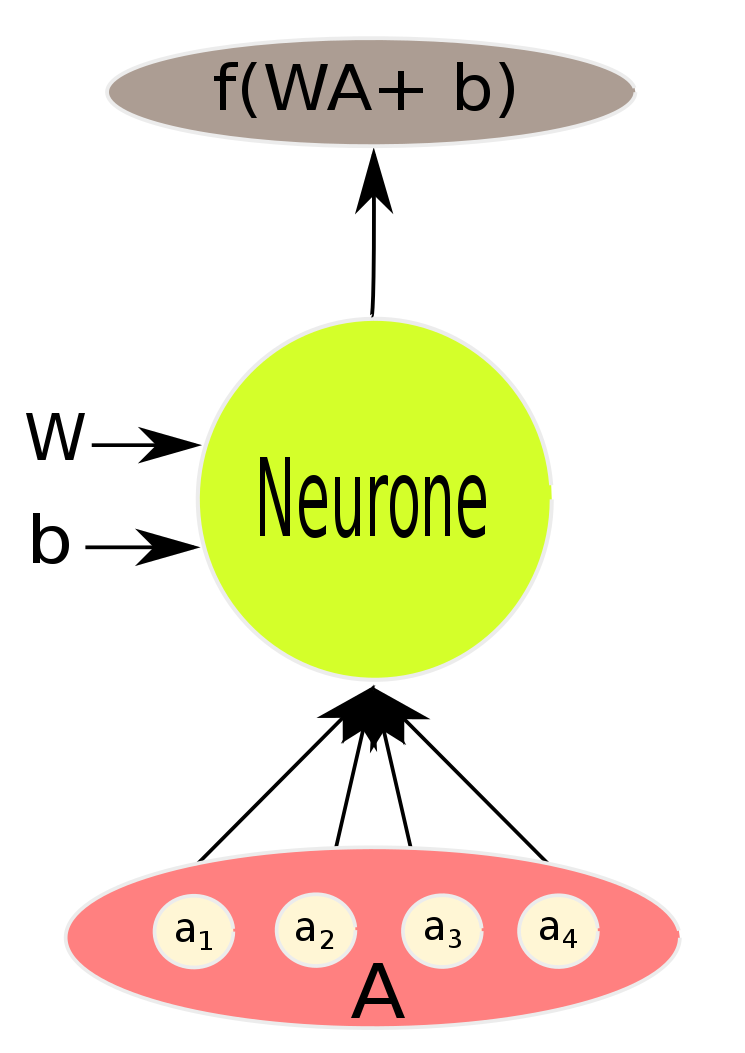
\includegraphics[width=0.9\textwidth]{Neuron}
    \caption{Exemple de neurone formel}
  \end{minipage}
  \hfill
  \begin{minipage}[b]{0.3\textwidth}
    \includegraphics[width=\textwidth]{Shallow}
    \caption{Réseau de neurones complètement relié non profond}
  \end{minipage}
  \hfill
  \begin{minipage}[b]{0.3\textwidth}
    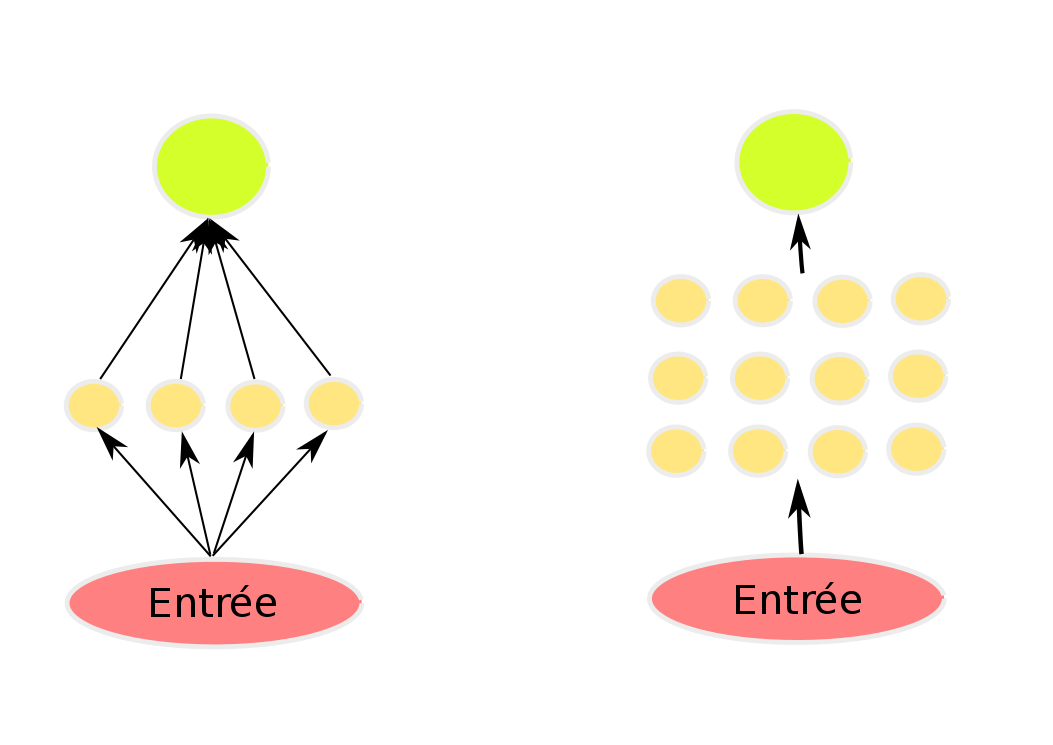
\includegraphics[width=\textwidth]{Deep}
    \caption{Réseau de neurones profond}
  \end{minipage}
\end{figure}


\subsection{Entraînement non supervisé}

\paragraph{Quel objectif poursuivre?}

Une grande problématique de l'apprentissage profond est le besoin d'accéder à de
grandes bases de données labelisées pour pouvoir entraîner les réseaux. Si cette difficulté
n'est plus d'actualité dans nombreux domaines, elle est indissociable de notre
étude des protéines. En effet, le nombre de protéines appartenant à une famille,
une super-famille ou une catégorie est limité. De fait, il n'est pas réaliste
d'espérer avoir assez de données pour exploiter les techniques d'apprentissage
purement supervisées. Comment faire pour demander à une machine de s'entraîner par elle même sans
qu'on lui dise quelle conclusion tirer à partir de son résultat? Une façon de
faire consiste à lui demander de retrouver son entrée. Ainsi, on ``encode''
l'information dans un premier temps, puis on la \og décode\fg : c'est l'auto-encodeur.

\paragraph{Donc on entraîne un réseau complexe à... retrouver l'identité?}

Ce n'est pas tant le but qui est intéressant ici, mais la façon de l'atteindre,
c'est-à-dire, la \textbf{représentation latente} acquise par l'encodeur.
Évidemment, il y a un réel risque que cette manière de l'atteindre ne soit pas
particulièrement intéressante non plus (on encode l'identité, puis on décode
l'identité). Pour éviter cela on dispose de plusieurs moyens:

\begin{itemize}
\item Forcer l'encodeur à encoder l'entrée en une représentation latente
  de dimension inférieure (\cite{hinton2006reducing}). Ainsi, on s'assure de ne pas pouvoir juste propager
  l'identité. Mieux encore, la représentation intermédiaire, ``condensée'' peut
  permettre de découvrir des ``points robustes'' de ce qu'on est en train
  d'apprendre.
\item Corrompre l'information donnée en entrée (comme proposé par
  \cite{Vincent:2008:ECR:1390156.1390294}) pour forcer l'encodeur à
  ``deviner'' ce qu'il manque, ce qui permettrait par exemple de mettre en
  lumière des corrélations non évidentes à l'oeil nu.
\item Poser des contraintes sur la représentation latente acquise,
  typiquement en forçant des objectifs de régularisation sur les paramètres.
\end{itemize}

\begin{figure}\centering
  \begin{minipage}{0.325\linewidth}
    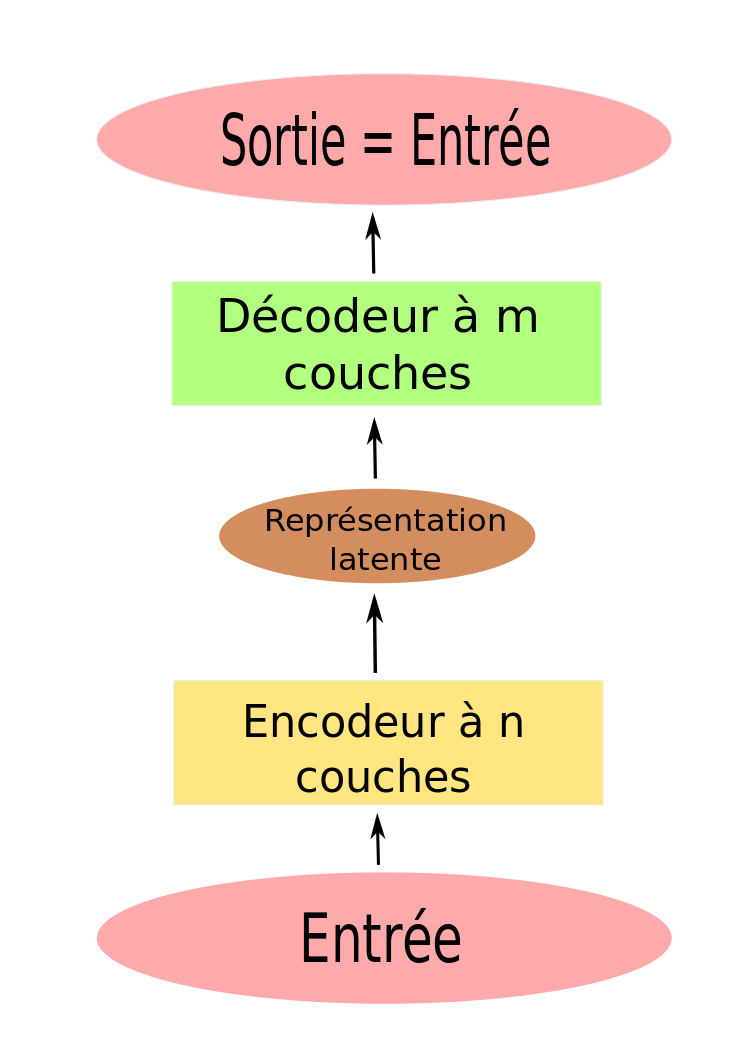
\includegraphics[width=\linewidth]{Autoencoder}
    \caption{Auto-encodeur classique}
  \end{minipage}
  \hfill
  \begin{minipage}{0.65\linewidth}
    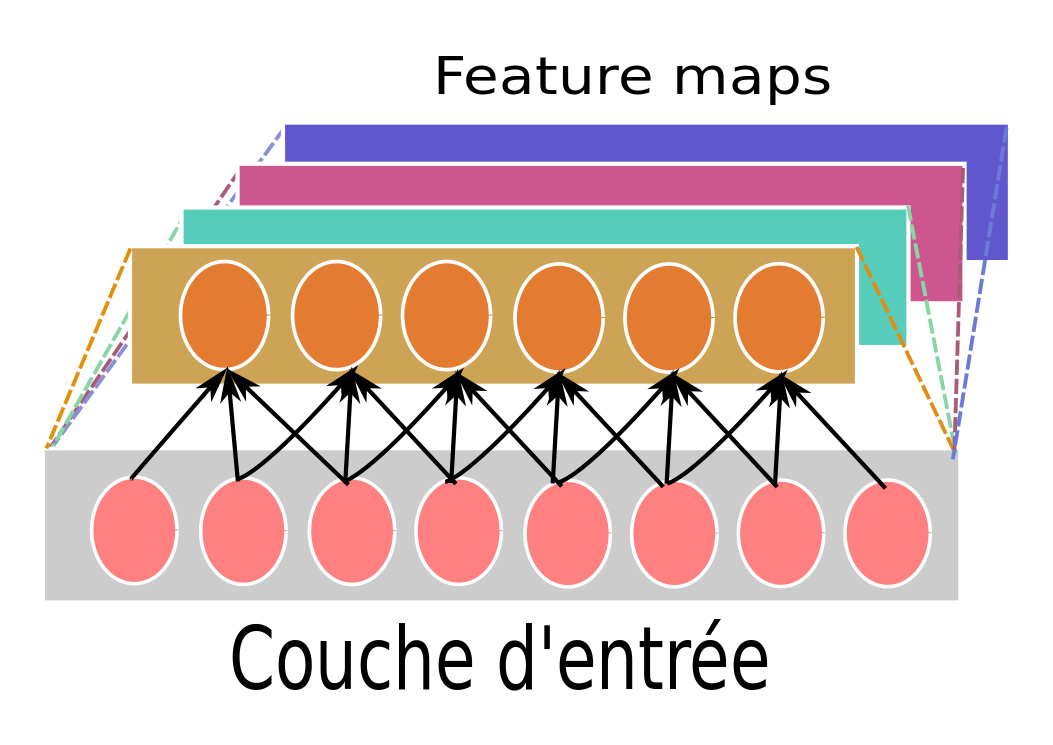
\includegraphics[width=\linewidth]{Conv}
    \caption{Exemple de couche convolutive avec des fenêtres de taille $1\times 3$}
  \end{minipage}
\end{figure}

\subsection{Réseaux convolutifs}

\paragraph{Il y a une marque caractéristique (feature) des images d'un certain type}

Cela est un élément utile à la reconnaissance d'images, mais il semble
difficile pour un réseau neuronal profond d'acquérir cette représentation par
lui-même. Ce qu'on peut faire par contre, est \og
scanner\fg sur une \og fenêtre\fg, par exemple des carrés $3\times 3$ de l'image en question à l'aide d'un filtre
permettant de décider si la marque apparaît dans le carré examiné. En pratique, c'est créer une couche cachée
dont chaque neurone applique une même fonction de transformation sur les 9 neurones d'un
carré $3\times 3$. Il s'agit donc de faire une convolution sur l'image d'une
fonction de transformation! Cette méthode reste applicable sur un chaîne de
caractère de longueur $n$, puisqu'il s'agit d'une image de taille $1\times n$ en
cherchant sur des fenêtres de taille $1\times 3$ par exemple.

Nous venons de décrire une couche générant une image réduite dont chaque
neurone/pixel donne la valeur de l'application d'une fonction à un carré
$3\times 3$. Nous appellerons une telle représentation \texttt{feature map}
(littéralement, carte de caractéristiques):
elle donne la représentation d'une \og feature\fg sur l'image. En un sens il
s'agit là d'une convolution puisqu'on prend une fonction (l'image
tridimensionnelle) et une autre \og pseudo-fonction\fg (le filtre de la
caractéristique étudiée, à la différence près que ce filtre est constant sur
l'espace étudié) et on effectue la convolution de ces deux fonctions
vectorielles.

\paragraph{Pourquoi s'arrêter à une \texttt{feature map}?}

Typiquement on crée plusieurs \texttt{feature maps} en parallèle (\textbf{Figure
5}) dans un réseau
convolutif (ou convolutionnel). Rappelons déjà que nous n'avons pas beaucoup de contrôle sur la
caractéristique que le réseau va retrouver puisqu'il va apprendre la
caractéristique qui donne le meilleur résultat par lui-même. Multiplier les
\texttt{feature maps} permet de distinguer plus de points caractéristiques qui
seront ensuite traités par une couche supérieure.

Si on veut rajouter une couche convolutionnelle au dessus, elle opérera non
seulement une opération sur un carré de chaque \texttt{feature map}, mais elle
effectuera une opération sur les résultats de cette opération sur chaque \texttt{feature
map} et les couches convolutives constituent le coeur de certains réseaux de
reconnaissance d'image (\cite{lecun1998gradient}).

% \paragraph{Réduire la charge de calcul}

% Pour augmenter un peu la robustesse du système à une translation par exemple, on
% effectue un \texttt{pooling} qui consiste à regrouper ensemble des blocs de
% neurones. Non seulement cela permet de réduire la taille de la représentation
% considérée, cela fait qu'une simple translation a moins de chance de changer
% quoi que ce soit à l'image obtenue après transformation.


% Une architecture typique se constitue donc d'un enchaînement de couches de
% convolution et de pooling, avec une ou plusieurs couches \og classiques\fg
% permettant de tirer une conclusion sur les informations récupérées. Une telle
% architecture est proposée dans \cite{lecun1998gradient} sous la forme du réseau LeNet5

\subsection{Réseaux récurrents}

Toutes les architectures proposées jusqu'à maintenant traitent l'entrée comme
une \og image\fg: il n'y a pas de notion d'ordre entre les différents éléments
de l'entrée. Une telle représentation est peu satisfaisante si on veut traiter
des suites d'entrées comme une phrase.

\paragraph{Il faut une architecture capable de tenir compte des entrées déjà lues}

On appelle réseau récurrent une unité  particulière qui prend en entrée une suite
d'éléments, et à chaque étape de calcul renvoi une sortie et un état caché
qu'il se renvoie dans une boucle de rétroaction. Ainsi, le traitement de
l'élément suivant de l'entrée dépend de celui de l'élément courant.

Si on \og déplie\fg l'exécution du problème, on réalise que la séquence passe en
fait par un nombre de couches cachées égal au nombre d'éléments dans la suite!
(\textbf{Figure 6})
Ainsi, nous avons établit un réseau qui est capable de traiter un élément d'une
suite en se rappelant en quelque sorte de ce qui s'est passé avant. La seule
question qui reste à traiter est le fonctionnement exact de la couche cachée.

Il est possible de faire fonctionner cette unité cachée comme un neurone classique avec une sortie et entrée supplémentaire
représentant l'état caché, mais cela pose des problèmes d'évanouissement du
gradient lors de la rétro-propagation. Une unité cachée qui résout ce problème et
est largement utilisée dans la littérature est l'unité LSTM (ou ses dérivatifs)
introduite dans \cite{hochreiter1997long} (\textbf{Figure 7}).

\begin{figure}[!tbp]
  \centering
  \begin{minipage}[b]{0.45\textwidth}
    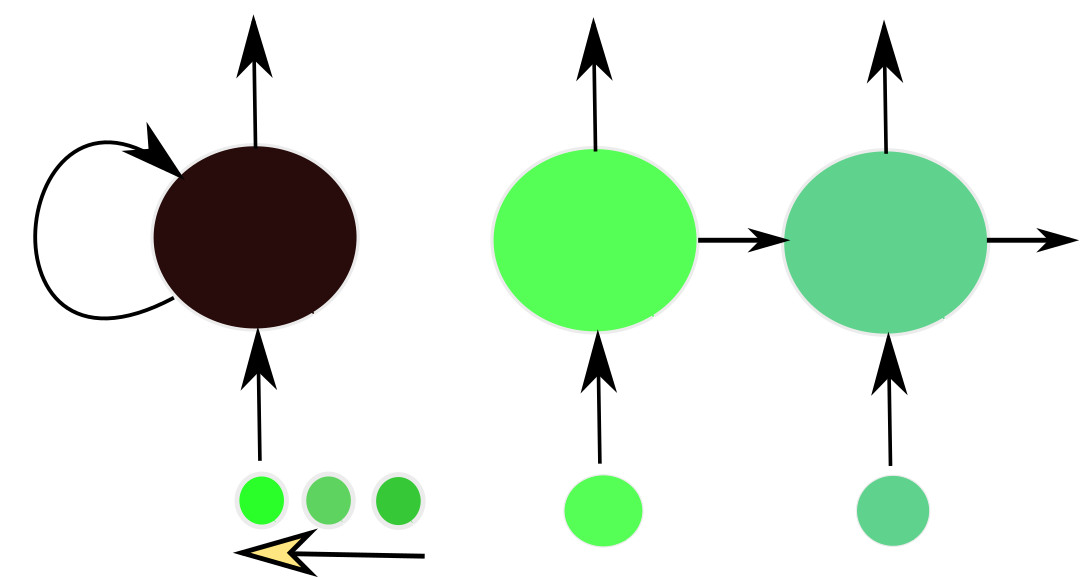
\includegraphics[width=\textwidth]{Recurrent}
    \caption{Réseau récurrent à gauche, forme dépliée temporellement à droite}
  \end{minipage}
  \hfill
  \begin{minipage}[b]{0.5\textwidth}
    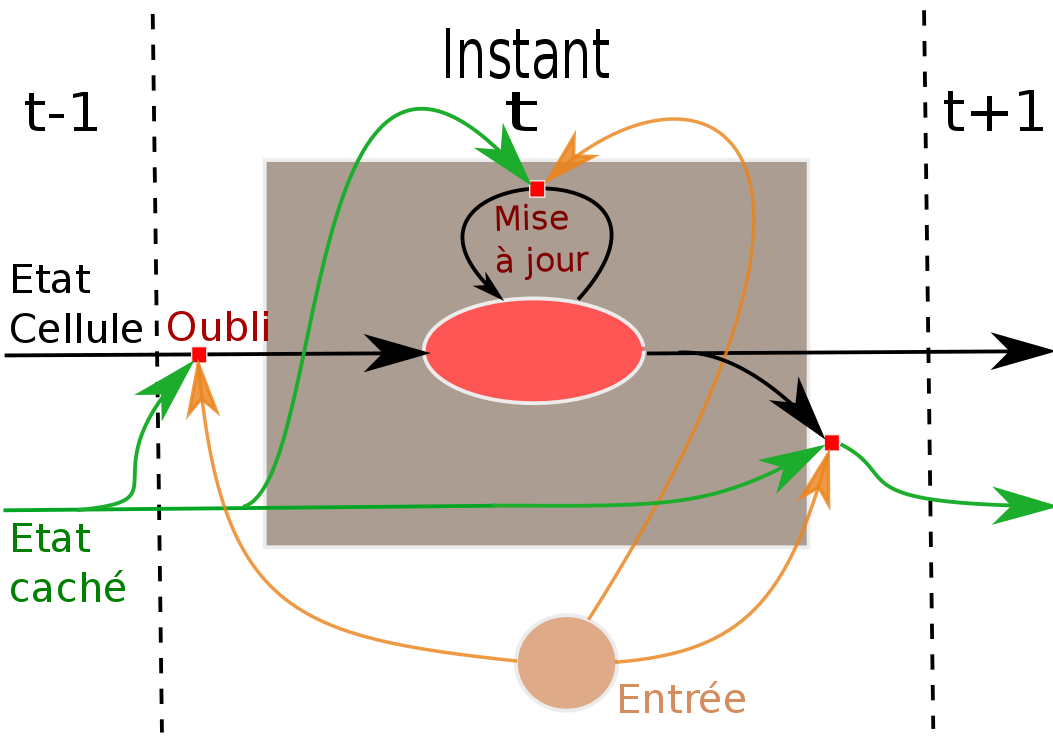
\includegraphics[width=\textwidth]{LSTM}
    \caption{Exemple d'unité LSTM}
  \end{minipage}

\end{figure}

\paragraph{Long Short-Term Memory (LSTM)}

L'idée est qu'on a un état de
cellule, un état caché et une entrée. A chaque passage dans la couche, on calcule
quel degré d'information il faut retenir de l'état de la cellule en fonction de
l'état caché et de l'entrée (porte d'oubli). Ensuite on calcule s'il faut ajouter de
l'information à l'état de la cellule (porte de mise à jour). Enfin, on fait le calcul de la sortie et
de l'état caché à partir des trois données précédentes.

% \paragraph{Pourquoi utiliser un réseau récurrent?}

% Les réseaux récurrents se sont avérés très utiles à l'étude du langage naturel
% puisqu'il permettent de détecter des corrélations dans une phrase qu'un réseau
% convolutionnel ne détecterait pas forcément (la fenêtre de détection d'une
% couche convolutionnelle est après tout de taille finie).  La sortie récupérée
% peut être de deux types différents: on peut récupérer la suite des sorties du
% réseau récurrent, ou on peut choisir de récupérer la dernière sortie de la
% couche récurrente qui servirait alors de \og résumé\fg de ce qui s'est passé à
% la lecture de la suite.

\paragraph{Un auto-encodeur récurrent?}

Les réseaux récurrents ont entre autres choses été grandement utilisés dans
l'étude de langages naturels. Une architecture d'encodeur-décodeur profonde que nous avons particulièrement étudié
(et qui fournit de bons résultats pour la détection de structures comme la copie
dans une chaîne) est celle proposée dans \cite{DBLP:journals/corr/ChoMGBSB14}.
L'idée est d'utiliser un premier auto-encodeur pour servir d'encodeur: on ne
récupère que sa sortie sur le dernier terme de la suite d'entrée. Cette sortie
est de dimension finie et nous servira de résumé (qui compresse éventuellement
l'information). Il suffit ensuite de passer ce résumé dans un autre
réseau récurrent en récupérant cette fois chaque sortie. Dans
l'article original, la sortie du décodeur au temps $t$ lui est aussi donné en
entrée au temps $t+1$, mais ce n'est pas le cas dans notre étude.

\subsection{Domaine d'étude: Protéines}

Notre étude s'est portée sur la façon d'appliquer les diverses techniques
précédemment mentionnées pour traiter le cas des protéines.

A l'instar d'une phrase qui est chaîne de mots, une protéine est une chaîne
d'acides aminés de longueur variable. Un acide aminé est une molécule chimique,
et de tels acides aminés interviennent typiquement dans les séquences
peptidiques. Ces acides ont chacun leur propriétés physico-chimiques
particulières comme leur hydropathie, leur charge électrique ou leur solubilité.

\paragraph{Structure primaire}

La séquence peptidique d'une protéine constitue ce qu'on appelle sa structure
primaire, mais une protéine ne peut pas se résumer à sa séquence peptidique.
C'est cette structure primaire que nous utiliserons en entrée de nos réseaux profonds.

\paragraph{Structure secondaire}

D'un point de vue local, les acides s'arrangent en des structures locales de
faibles dimensions telles que des hélices-$\alpha$ (constituées de 3, 4 ou 5 tours
d'hélices), de brins-$\beta$ ou d'autres structures tels que des retournements.
On parle alors de structure secondaire de la protéine. La grande majorité des
travaux existants sur l'application de techniques d'apprentissage profond au
séquences peptidiques traitent de la prédiction de structures secondaires
(\cite{Spencer:2015:DLN:2817095.2817106}) ou d'autres caractéristiques locales (\cite{qi2012unified}).

\paragraph{Structure tertiaire}

La façon dont l'ensemble de ces acides et structures locales s'organisent dans
l'espace constitue la structure tertiaire de la protéine. On peut décomposer la
classe structurale (répertoriée par \cite{fox2014scope} par exemple) de la protéine à partir de la structure secondaire:
$all-\alpha$, $all-\beta$, $\alpha /\beta$, $\alpha + \beta$,
$peptide$, ... Il n'existe à notre connaissance que peu de travaux tentant
d'appliquer les techniques d'apprentissage  profond à la prédiction de classes
structurales (\cite{jian2013predicting}) en effectuant un simple pré-entraînement par
empilement d'auto-encodeurs.

\paragraph{Domaines}

Nous n'avons cependant pas étudié les séquences peptidiques entières des
protéines. Une façon de voir les choses est de dire que les protéines sont des
assemblages de chaînes, généralement assez longues, d'acides aminés. En faisant
des études d'alignement sur les séquences peptidiques, il est possible de
remarquer que des même chaînes longues apparaissent dans différentes protéines.
On parle alors de domaine pour désigner cette chaîne.
 La grande majorité de notre travail s'attache à
étudier ces domaines, bien qu'il ait fallu trouver des moyens de contourner les
problèmes posés par la longueur malgré tout importante de tels domaines. 

\subsection{Initialisation et optimisation des réseaux d'apprentissage profond}

\paragraph{Entraînement non-supervisé?}

Il a été montré dans de nombreux travaux qu'il est possible d'entraîner des
auto-encodeurs les uns à la suite des autres et d'aboutir à des situations permettant
d'éviter de trop mauvais minima locaux. C'est d'ailleurs ce qui a motivé le
second souffle de l'apprentissage profond vers la fin des années 2000

Néanmoins, des travaux plus récents ont montré qu'il suffit d'utiliser des
initialisations aléatoires bien choisies pour largement passer outre les problèmes
de minima locaux quand l'ensemble d'apprentissage est de taille élevée. Cependant, nous avons aussi dû travailler avec des jeux de
données de taille faible, ce qui a nécessité le passage par de l'apprentissage
non-supervisé pour les tâches de classification où peu d'exemples labélisés existent.

\paragraph{Rétropropagation}

Nous disposons d'une évaluation (fonction) de la qualité de la décision prise en fin de réseau. Notre but est de
minimiser cette fonction en modifiant les paramètres internes du réseau (qui
déterminent les transformations effectuées sur l'entrée.). Pour ce faire, on
utilise typiquement le gradient de la fonction de coût. Cela peut se faire au
travers de quelque chose d'aussi simple que la descente de gradient stochastique, mais cette
dernière a de nombreux défauts. Dans cette article nous utiliserons les
optimisations dites \texttt{adagrad} (\cite{duchi2011adaptive}) (très efficace dans les réseaux
convolutifs) et \texttt{RMSProp} (\cite{hintonlecture}) (très efficace dans les réseaux récurrents).

\paragraph{De la non linéarité}

En un sens, les réseaux neuronaux cherchent à observer les données \og sous un
certain angle\fg qui permet de trouver des corrélations: cela permet de faire de
la classification, de la reconstruction, voire de la prédiction. Néanmoins si on
se borne à effectuer des opérations linéaires (sommes pondérées
d'entrées, transformations affines) il est tout a fait possible de passer à coté
d'un regroupement intéressant des points (les fonction linéaire préservent
notamment l'alignement ce qui peut se révéler être un grand problème). De fait,
il y a toujours \og à la fin\fg d'une couche une fonction dite \og
d'activation\fg qui opère une transformation non-linéaire sur la sortie.
Traditionnellement, on applique une sigmoïde ou une tangente hyperbolique, mais
Hinton a montré qu'il est plus judicieux pour des raisons d'écrasement ou
explosion de gradient d'utiliser une fonction de seuillage
\texttt{ReLU} (Rectified Linear Unit, \cite{glorot2011deep}).

\paragraph{Éviter le sur-apprentissage}
  
On peut aléatoirement désactiver certains neurones, ce qui force le système à
 éviter de spécialiser le réseau sur l'ensemble d'entraînement et non sur
le domaine où on veut l'appliquer (\cite{srivastava2014dropout}). Il est raisonnable qu'un réseau
entraîné sur des familles de protéines gère mal les chaînes purement
aléatoires, mais il serait problématique qu'il n'arrive pas à
traiter des protéines proches des exemples d'entraînement mais n'en faisant
pas partie. En effet, si on veut catégoriser les pompiers, et que par hasard
tous ceux de l'exemple d'entraînement sont bruns, il y a un risque d'associer
pompier et brun.

L'idée est la suivante: s'il est autorisé de copier sur ses camarades à un
examen, et qu'il est connu qu'un élève aura 20 à l'épreuve, un comportement
possible est de ne rien faire et simplement compter sur l'élève qui travaille.
Cela est problématique car on dépend alors uniquement du résultat de cet
élève/neurone, et la perception des choses qu'on a est fortement biaisée par ce
que ce neurone sait. La solution adoptée revient à annoncer qu'un certain
pourcentage de la classe sera malade le jour de l'examen, ce qui force tout le
monde à apprendre. Un telle approche est appelée \textbf{dropout}, et la
proportion de neurones neutralisés pendant l'entraînement est un paramètre fixé
par l'expérimentateur.

Il a néanmoins été montré dans \cite{gal2015theoretically} qu'une telle
architecture est complètement inutile dans le cas des réseaux récurrents.
Néanmoins, il y est proposé d'effectuer un oubli dans la dépendance temporelle
du réseau (c'est à dire au niveau de l'état caché) ce qui permet d'obtenir des
résultats similaires à la technique précédente pour des réseaux classiques.

\section{Etude réalisée}
\label{sec:etude}

\subsection{Matériel}

Nous avons effectué l'ensemble de nos travaux à l'aide librairies du langage de
programmation Python (\url{http://www.python.org}).

Pour ce qui est de l'aspect apprentissage profond, nous avons principalement
utilisé \texttt{keras} (\cite{chollet2015keras}) qui est une libraire haut niveau
permettant de manipuler facilement des couches d'apprentissage. Ce choix vient
d'une part de la nature des problèmes étudiés qui nous mènent à tenter
l'utilisation de plusieurs architectures (ce qui invalide des librairies plus spécialisées) et de l'autre de la grande
souplesse offerte par Keras. En effet, \texttt{keras} peut utiliser deux
librairies bas niveau python (il est possible de choisir entre les deux): la
librairie académique \texttt{Theano} (\cite{2016arXiv160502688full}) et le plus récent
\texttt{Tensor Flow} (\cite{tensorflow2015-whitepaper}) de Google.

Pour ce qui est de la manipulation de séquences peptidiques à proprement parlé,
nous avons utilisé des données de la base de donnée \texttt{SCOPe}
(version 2.6, séquences à 40\% d'identité ou moins, \cite{fox2014scope}) et la librairie python Biopython (\cite{Cock01062009},
\cite{hamelryck2003pdb}). L'outil DSSP (\cite{kabsch1983dictionary}) a aussi été
utilisé pour établir la structure secondaire des protéines étudiées.

\subsection{Représentation des chaînes peptidiques}

La tâche globale que nous nous sommes fixés dans une première approche est la
prédiction de classe structurale. Ce qui a été fait à de maintes reprises par le passé est la représentation des
protéines non pas comme chaînes d'acides, mais comme un vecteur dépendant de
différents paramètres. Ces paramètres vont de notions simplistes comme le nombre
d'occurrences de chaque acide aminé dans la chaîne à des considérations beaucoup
plus complexes comme l'étude des fonctions de la protéine. L'état de l'art donne
une précision de l'ordre de 98\%, mais exploite la connaissance d'un grand
nombre de caractéristiques fonctionnelles des protéines concernées, ce qui
limite l'intérêt de l'approche. \cite{jian2013predicting} utilise une
représentation n'exploitant pas ces caractéristiques, mais renonce tout de même
à travailler sur la séquence peptidique en invoquant un problème de généralisation.

Notre travail s'est principalement basé sur l'étude de protéines en tant que
chaîne d'acides aminés représentés par des lettres. En quelque sorte, nous traitons donc des suites de \og
mots\fg. De fait, il est nécessaire de déterminer une façon de représenter ces
différents mots. Il est facile de voir pourquoi la première idée de simplement
indexer les acides par des entiers est problématique: pourquoi la lettre \og
A\fg serait elle plus proche du \og B\fg que du \og Z\fg? Pour résoudre ce
problème, nous nous sommes intéressés à ce qui a été fait en traitement de langages
naturels.

\paragraph{Représentation one-hot}

Une représentation répandue, bien qu'assez simpliste consiste à créer un espace
contenant autant de dimensions qu'il y a d'acides aminés et représenter chaque
acide aminé par un vecteur d'une base orthogonale de cet espace. Plus
simplement, cela veut dire qu'on représente chaque acide par un vecteur ne
contenant que des 0 et un 1. Cette représentation \texttt{one-hot} permet d'avoir des résultats,
mais elle présente en langage naturel l'inconvénient d'engendrer une
représentation dans l'espace très lacunaire, ce qui crée des espaces inutilement
grands. Ce problème est secondaire dans notre cas puisqu'il n'y a qu'une
vingtaine d'acides à considérer.

\paragraph{Représentation distribuée et représentation experte}

Néanmoins, il est intéressant de remarquer que des outils ont été inventés en
langages naturels pour passer outre ce problème. L'idée est d'apprendre une
représentation distribuée de dimension inférieure prenant en compte les mots
apparaissant généralement avec celui considéré. Cela se fait avec des techniques
d'apprentissage qui cherchent à maximiser le score de phrases valides et
minimiser celui de phrases non valides. Ces techniques ne sont pas applicables à
notre problème à cause de la façon dont les séquences peptidiques fonctionnent,
mais nous avons voulu retenir l'idée qu'on peut placer les acides dans un espace
de dimension faible en tenant compte de leur spécificités. En regardant 4
propriétés physico-chimiques, nous avons donc créé une telle représentation.
L'aspect important d'une telle représentation est qu'elle permet de justifier du
fait que deux acides sont proches du point de vue de leur représentation, ou du
fait que trois acides sont équidistants. En effet, la représentation précédente
posait le problème inverse de l'indexage: pourquoi tous les acides seraient-ils équidistants?

\subsection{Choix des types d'architectures d'apprentissage profond}

Nous avons précédemment inventorié différentes architectures d'apprentissage
profond, et nous allons maintenant expliquer pourquoi celles que nous avons
choisis d'utiliser semblent adaptées au problème étudié.

Dans le cadre du traitement de séquences peptidiques, il semble tout indiqué
d'utiliser des réseaux récurrents puisqu'une structure temporelle semble
apparaître dans l'enchaînement des acides aminés. Néanmoins, le grand défaut de
réseaux récurrent est que, contrairement aux réseaux profonds dits \og
classiques\fg, ils repèrent des dépendances temporelles et non hiérarchiques.
Pour pallier à ce problème, il semble nécessaire d'empiler les réseaux
récurrents, ce qui a vite des conséquences significatives en termes de temps de
calculs dès qu'on traite des séquences un peu longues.

Une autre architecture intéressante est celle des réseaux convolutionnels
exposés plus haut. Dans la façon de procéder décrite plus haut, un acide aminé
est traité comme un \og mot\fg. Cela ne correspond pas nécessairement à une
quelconque réalité, à moins qu'on pense qu'une lettre est un mot. Il n'existe
cependant pas de moyen d'extraire à priori un \og mot\fg (un groupe d'acides)
d'une chaîne peptidique: il n'y a pas d'acide \og séparateur\fg. Cependant, les
réseaux convolutionnels offrent un moyen alternatif de repérer ces mots: si une
\texttt{feature map} est appliquée sur 7 acides, alors cette \texttt{feature
  map} sera capable de repérer (après entraînement) un mot (caractéristique) de
longueur inférieure ou égale à 7.

En outre, l'idée de pouvoir utiliser une \og fenêtre glissante\fg pour étudier
des fragments d'une chaîne plus longue a été préservée.

\subsection{Etude préliminaire sur séquences artificielles}

Afin d'orienter notre recherche sur les séquences peptidiques et mieux comprendre le fonctionnement des réseaux neuronaux et leurs
comportements face à différentes situations, nous avons procédé à quelques
expérimentations préliminaires sur deux types de tâches: un entraînement
d'autoencodeurs et un entraînement de classificateur.

Nous avons généré aléatoirement plusieurs jeux de données pour comparer les
capacités de diverses architectures d'auto-encodeurs et classificateurs. Nous
avons testé deux types de jeux de données: un jeu de données où la première
moitié de la chaîne est fixée et où la seconde moitié est telle que chaque
lettre est tirée avec probabilité uniforme; et un jeu de données où la première
moitié est tirée avec probabilité uniforme sur chaque lettre et où la seconde
moitié est égale à la première moitié.

\subsubsection{Auto-encodeurs}

Nous envisageons principalement deux architectures d'encodeurs: un réseau
convolutionnel (à couches multiples) et un réseau récurrent LSTM (à une ou plusieurs
couches) dont nous récupérons la dernière sortie. Le décodeur est dans tous les
cas un réseau récurrent LSTM.

Les deux architectures n'ont aucun problème à repérer la caractéristique des données dont le
début est fixé, ce qu'elle reconstitue très bien. Par contre, il semble que l'architecture dont l'encodeur est un
réseau convolutionnel ne parvient pas à décoder correctement les caractères
aléatoires. De plus, il ne semble même pas repérer la relation de \og copie\fg
présente dans le second jeu de données. Au contraire, il semble que l'encodeur
récurrent, même à une seule couche apprend très vite à créer des mots dont les
deux moities sont très similaires, même si elles n'ont pas grand chose à voir
avec l'entrée réelle. Sous condition de disposer d'un temps d'entraînement assez
long, l'encodeur récurrent permet aussi de reconstituer correctement les
caractères tirés aléatoirement.

\subsubsection{Classificateurs}

Nous avons étudié deux architectures de classificateurs, qui correspondent
principalement à l'encodeur (non pré-entraîné) des auto-encodeurs précédents auxquels un neurone
final est ajouté pour prendre la décision finale de classification. Le jeu de
donnée fourni correspondait à une moitié de chaînes suivant une règle spécifique
(premières lettres fixes ou copie), et d'une moitié de chaînes purement
aléatoires. L'objectif était de savoir si le classificateur était à même de
repérer des corrélations entre différentes positions.

La classification fonctionne bien dans les deux cas. De manière assez
intéressante, cela veut dire que les réseaux convolutionnels sont bien capables
de reconnaître les ``points caractéristiques'' de chaînes de caractères, mais le
décodeur récurrent n'est pas capable de reconstituer la chaîne à l'aide de
l'information contenu dans la représentation latente. Il est à noter cependant
que les minima locaux ont présenté un problème avec une initialisation
aléatoire uniforme simple, puisque le classificateur avait tendance à toujours
répondre la même chose. On constatait donc un point de selle de la fonction à
minimiser par le réseau.

% \subsection{Clustering de protéines}


% En première approximation, on pourrait penser retrouver un hyperplan ou une
% nappe aparentable à une feature connue. Néanmoins une telle étude est difficile
% à exploiter. Nous nous sommes penchés sur la piste du clustering
% de protéines en fonction de leur représentation intermédiaire. En effet, si on
% regroupe ensemble des protéines \og proches\fg du point de vue de leur
% représentation intermédiaire, il est peut-être possible de remarquer
% des points remarquables dans la structure de protéines qui pourront être
% ré-utilisés de manière indépendante de l'apprentissage profond plus tard.

% Un simple algorithme de K-means permet de faire le découpage en parties de
% l'ensemble d'apprentissage. Pour étudier les différentes parties de l'espace
% latent ainsi découpées, on procéde à une analyse de la fréquence d'apparition de
% fragments d'un domaine donnée (c'est-à-dire le rapport entre le nombre
% d'apparitions dans le groupe et le nombre de fragments totaux du domaine, afin
% d'éviter d'introduire un biais favorisant les domaines longs) et à une étude du
% nombre fragments comprenant uniquement des acides faisant partie d'une
% hélice-$\alpha$ ou d'une feuille-$\beta$

\subsection{Étude de la corrélation de paramètres}

Les auto-encodeurs que nous avons entraîné génèrent une représentation intermédiaire dans un premier
temps. Nous avons voulu étudier cette représentation intermédiaire pour en
apprendre plus sur les choses auquelles l'auto-encodeur fait attention quand il
encode la protéine et qui lui permettent de reconstruire par la suite la
protéine. \cite{jian2013predicting} a déjà effectué une étude sur la capacité de réseaux d'auto-encodeurs
empilés à classifier la structure secondaire de protéines, mais cette étude ne
s'est malheureusement pas attardée sur le problème de la représentation
intermédiaire.

Une première étude sur la façon dont les représentations latentes se
regroupaient dans l'espace avec des méthodes de clustering ne s'est pas avérée
révéler un quelconque critère d'ordonnancement des fragments. 
Une façon de relever des caractéristiques sur la représentation
intermédiaire acquises est d'étudier les corrélations existant entre ses
caractéristiques et des paramètres liés au fragment de protéine étudiés. Nous
avons décidé d'étudier les paramètres de la représentation intermédiaire
suivants: sa norme, ses coordonnées dans l'espace latent et la distance entre la
représentation latente de deux fragments. De fait, il a fallu distinguer deux
types de données pour effectuer l'étude des corrélations puisqu'il a fallut
étudier des caractéristiques propres à un fragment, et des caractéristiques
d'un couple de fragments.

\paragraph{Paramètres d'un unique fragment}

Pour ce qui est des caractéristiques propres à un fragment, nous avons étudié
son hydropathie moyenne, sa charge moyenne, la présence d'acides aminés dans la
chaîne peptidique (regroupés en 5 catégories: Aliphatic, Aromatic, Neutral,
Acidic, Basic) et le fait que la chaîne est uniquement composée d'acides appartenant à
une hélice-$\alpha$ ou à une feuille-$\beta$. Ce dernier point a été fait à
l'aide l'outil DSSP introduit au début de cette section.

\paragraph{Paramètres d'un couple de fragments}

Nous avons fait l'étude, en outre de la distance entre les représentation
latentes, du score d'alignement entre les fragments (global et local) et du score de super-imposition structurale (relativement
aux $carbones-\alpha$, \cite{hamelryck2003pdb}).

\section{Expériences et évaluation}
\label{sec:exp}

\subsection{Auto-encodeurs}

\subsubsection{Modèles entraînés}

Les chaînes protéiques étudiées sont longues (jusqu'à 300 caractères). Les
auto-encodeurs sont entraînés non pas sur les chaînes protéiques mais sur des
fragments de chaînes peptidiques de taille 11, ce qui facilite les calculs et
correspond à une fenêtre permettant d'observer quelques structures secondaires.
De plus, cela présente l'avantage significatif d'augmenter très
significativement le nombre d'exemples d'entraînement disponibles, ce qui est
très important en apprentissage profond. 

Les auto-encodeurs décrits dans l'étude
préliminaire sont ceux qui ont été employés à nouveau dans cette étude des
fragments. Il peut paraître surprenant d'utiliser l'auto-encodeur convolutionel
ici alors qu'il n'avait pas réussit à accomplir sa tâche désigné. Néanmoins,
cela ne veut pas dire qu'il n'a pas pu apprendre de représentation intermédiaire
intéressante. Ainsi, nous avons tout de même entraîné un auto-encodeur
convolutionel dans l'espoir de pouvoir en faire une étude par la suite. Deux
représentation ont été employées pour les acides aminés: celle basées sur les
caractères physico-chimiques décrite plus haut pour l'auto-encodeur récurrent, et
une représentation \texttt{one-hot} pour les deux architectures proposées.

Les entraînements ont été effectués sur 100 \texttt{epochs} (cycle
d'entraînement sur les exemples) pour les représentations \texttt{one-hot} et 30
\texttt{epochs} pour la représentation experte avec des paramètres de \texttt{dropout} de 0.1
à chaque fois. Les encodeurs récurrents sont constitué de 3 réseaux récurrents
projetant l'entrée dans un espace latent de dimension 20 pour la représentation
\texttt{one-hot} et 50 pour la représentations experte,
tandis que l'encodeur convolutionnel est constitué de 5 couches convolutionnelles
de paramètres précisés en annexe. Le décodeur est à chaque fois constitué d'un
réseau récurrent simple.

\subsubsection{Pertinence de la reconstitution}

L'entraînement de l'auto-encodeur récurrent à représentation \texttt{one-hot} a rapidement donné des résultats très
satisfaisants en termes de reconstitution des fragments  avec une représentation
latente de dimensions raisonnablement faible (20 dimensions). L'entraînement des
autres auto-encodeurs a par contre nécessité plus d'efforts, dont une
initialisation aléatoire pertinente du réseau.

Un gros problème dans notre approche est qu'il n'est pas suffisant de savoir que
l'auto-encodeur apprend bien quelque chose, il faut aussi vérifier qu'il apprend
bien quelque chose sur la structure de fragments issus de protéines et non par
sur les chaînes de longueur 11 de manière générale. Si la représentation acquise
concerne les chaînes de longueur 11 en général, cela ne voudra cependant pas dire que les
données obtenues par la suite sont complètement inexploitables. En effet, il
n'est pas impossible que l'agencement des acides aminés obéisse à des règles
plus générales.
Une façon de vérifier les
choses et de tester une tâche de classification comme envisagé plus tôt. Si
les résultats obtenus mettent en évidence une amélioration avec le pré-entraînement, cela suggérerait que la représentation
obtenue est au moins exploitable pour l'apprentissage sur des fragments de
protéines. 

Une autre façon de procéder serait de vérifier le taux d'acides
devinés correctement par l'auto-encodeur et comparer ces taux entre les résultats
obtenus sur des éléments de l'ensemble de validation et ceux obtenus sur des
chaînes générées aléatoirement.
Malheureusement, une telle approche n'est possible que dans le cas des
auto-encodeurs récurrents sur une représentation \texttt{One-hot}. Dans les
autres cas, la représentation obtenue n'est de toute façon pas assez proche de
celle attendue pour avoir une réponse à notre interrogation. De plus, le
problème soulevé est nettement moins préoccupant dans le cas de la
représentation physico-chimique puisque l'apprentissage se fait sur un alphabet
\og spécialisé\fg de toute façon. Les résultats obtenus sur un auto-encodeur
récurrent sur représentation \texttt{one-hot} montre une amélioration de
performance de $50\%$ selon le critère avancé. Cette amélioration est cependant
 moins nette (de l'ordre de 6\%) quand on élimine des situations
problèmatiques - des caractères apparaissant rarement - pour l'autoencodeur,
mais laisse tout de même penser qu'un mécanisme d'inférence apparaît durant l'entraînement.

\subsubsection{Corrélations}

Les cartes de corrélations obtenues sont présentées dans ce rapport en annexe à
l'exception de celle pour des fragments individuels dans le cas de
l'auto-encodeur récurrent à représentation \texttt{one-hot} (\textbf{Figure 8}) jugée représentative des
résultats obtenus.

\paragraph{Etude de fragments individuels}

Une étude des corrélations entre les paramètres propres à la représentation
latente obtenue par l'encodeur et les caractéristiques physico-chimiques des
fragments considérés suggère plusieurs choses:
\begin{itemize}
\item Les représentation latentes (dans un espace de dimension 20) sont
  principalement réparties dans un espace bi-dimensionnel. En effet, la norme ne
  semble corrélée qu'à 4 dimensions, et il y a parmi ces 4 dimensions 2 paires
  de dimensions fortement corrélées. Cela suggère donc la mise en évidence d'un
  espace de plus faibles dimensions repéré par l'auto-encodeur qui à partir d'un espace de dimensions
  $26\times 11= 286$ injecté dans un espace de dimension 20 crée une
  représentation concentrée dans un espace presque bi-dimensionnel.
\item On semble remarquer une certaine corrélation entre la norme, une dimension
  de la représentation latente, et l'hydropathie moyenne du fragment. Cela
  suggère que l'hydropathie moyenne du fragment est un facteur discriminant
  permettant de bien différencier les fragments (en tant que chaînes
  peptidiques) entre eux.
\item On observe un phénomène similaire pour la charge moyenne du fragment, bien
  que cette fois la corrélation ne se fait qu'avec une dimension de la
  représentation latente, et non pas avec la norme elle-même.
\item En revanche, les résultats sont moins clairs pour ce qui est des
  caractéristiques liées aux structures secondaires qui présentent peu, ou pas,
  de corrélation avec la représentation latente acquise par l'encodeur
  récurrent. 
\item Les corrélations sont beaucoup plus faibles avec la représentation \og
  experte\fg discutée, ce qui pose des questions quand à ce qui est réellement
  appris par l'encodeur dans ce cas.
\end{itemize}

\begin{figure}
  \centering
  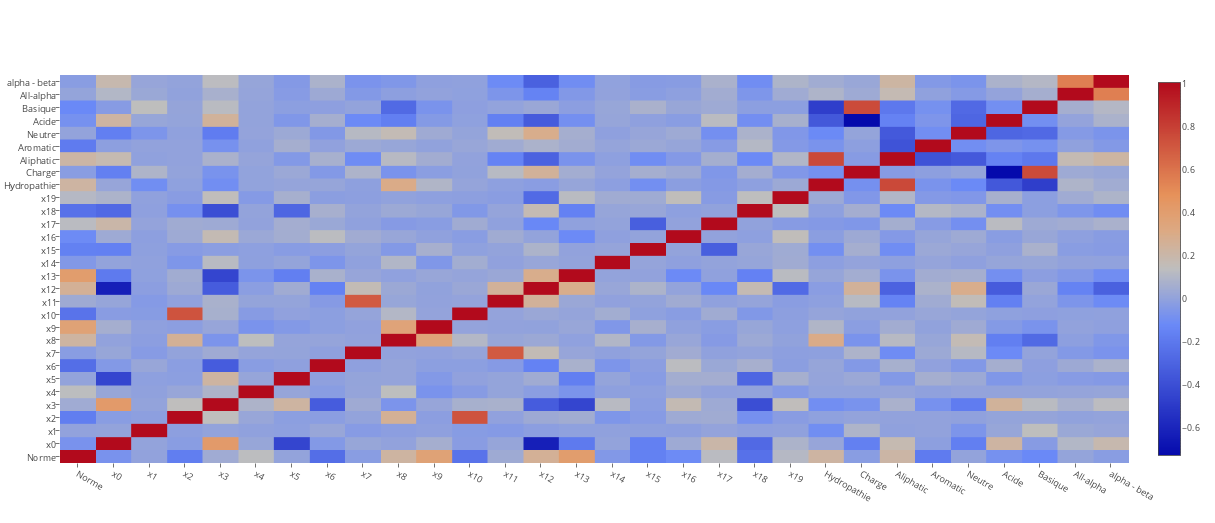
\includegraphics[scale=1.7]{SingleOneRecHeatf}
  \caption{Carte de corrélation sur les fragments individuels}
\end{figure}

\paragraph{Étude sur des paires de fragments}

L'étude sur des couples de fragments ne s'est par contre pas avérée mettre en lumière
une quelconque corrélation, si ce n'est que l'alignement structural entre deux
fragments est légèrement moins décorrélé de leur distance que leur score d'alignement
séquentiel. Il est remarquable que ce ne soit pas le cas. Dans le processus \og
d'embedding\fg en langage naturel, la représentation extraite garde des
propriétés de translation relative à des relations sémantiques (comme une
translation fixe entre féminin et masculin). 

\begin{wrapfigure}{R}{0.5\textwidth}
  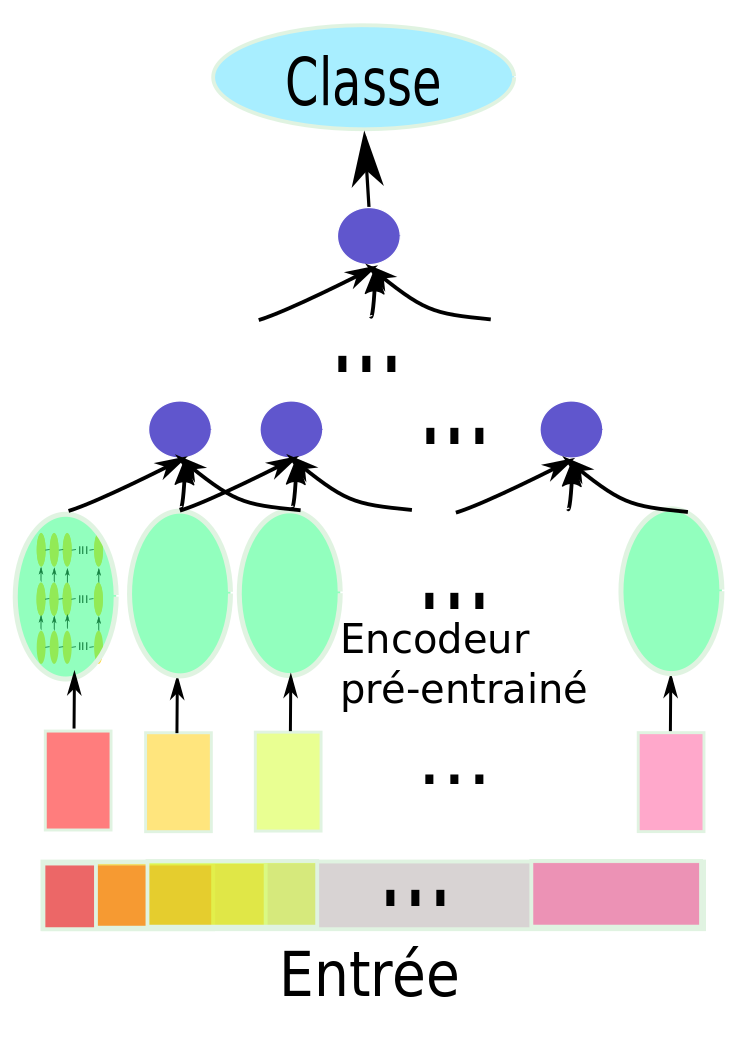
\includegraphics[width=0.45\textwidth]{Classd}
  \caption{Classificateur employé (avec encodeur récurrent)}
\end{wrapfigure}

Si le procédé d'acquisition de cette
\og représentation\fg (qui n'est ni plus ni moins qu'une représentation latente) ne
se fait pas exactement par auto-encodage, l'embedding acquis demeure une
représentation utile à l'apprentissage profond.  Il n'aurait donc pas été
absurde d'espérer voir une relation similaire apparaître dans le cas de notre
représentation intermédiaire sur les fragments de protéines. L'absence de telle
relation pourrait indiquer que, du point de vue de l'auto-encodeur du moins, une
telle information est d'importance secondaire pour l'encodage et décodage des protéines.

\subsection{Classificateur}

\subsubsection{Modèle entraîné}

Pour le classificateur, nous avons
utilisé l'encodeur de l'auto-encodeur précédent comme ``fenêtre glissante''
avant de décider avec un neurone final. L'idée est que pour chaque facteur de
taille 11 d'une chaîne peptidique, on applique l'encodeur de l'auto-encodeur
entraîné de manière non supervisée (\textbf{Figure 9}). De cette manière, nous espérons éviter
autant que possible une mauvaise initialisation du réseau comme décrit dans \cite{vincent2010stacked}

Le classificateur en lui-même dispose de 4 couches (dont le détail des
paramètres est donné en annexe) et le \texttt{dropout} est encore fixé à 0.1.

\subsubsection{Améliorations de performances par pré-entraînement}

\begin{figure}[!tbp]
\centering  
  \begin{minipage}[b]{0.45\textwidth}
    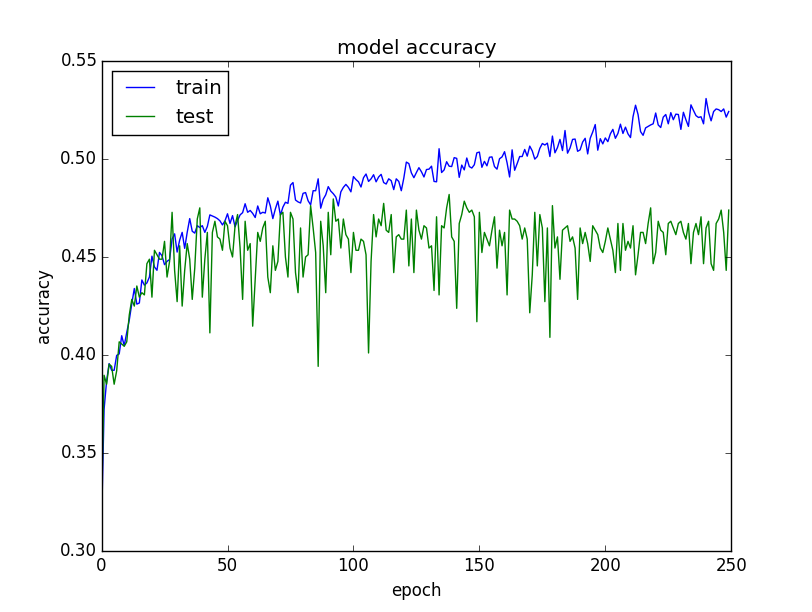
\includegraphics[width=1.2\textwidth]{SupClass}
    \caption{Performance pour le classificateur non pré-entraîné}
  \end{minipage}
  \hfill
  \begin{minipage}[b]{0.5\textwidth}
    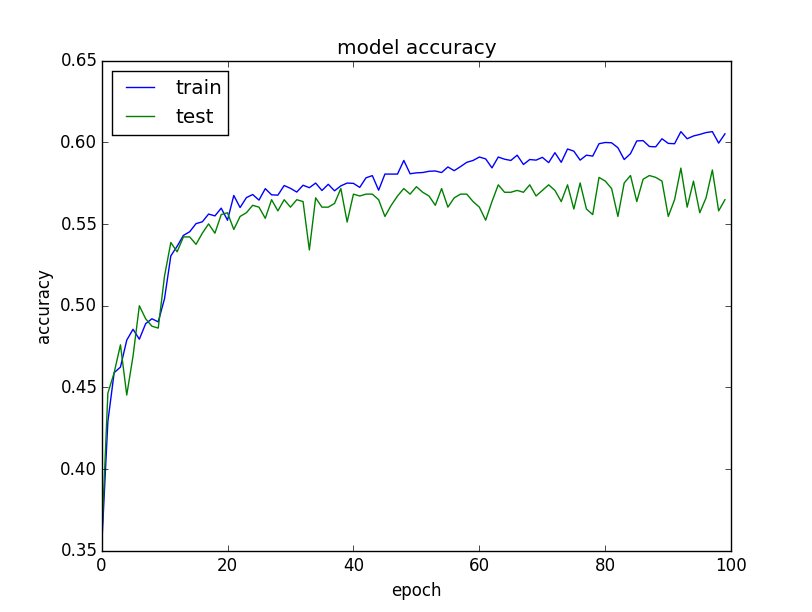
\includegraphics[width=1.1\textwidth]{SpeClass}
    \caption{Classificateur pré-entraîné avec encodeur
      récurrent à représentation one-hot}
  \end{minipage}
\end{figure}

On constate dans tous les cas une amélioration nette de la performance du
classificateur pré-entraîné (\textbf{Figure 10 et 11}, voir annexe pour
l'encodeur convolutionnel). Non seulement la précision de la classification
s'améliore plus rapidement, mais la précision limite atteinte est
significativement meilleure (une amélioration de l'ordre de 25\% est détectée
pour l'encodeur récurrent à représentation \texttt{one-hot}). De plus, il est
intéressant de noter un \og décrochage\fg entre la précision d'entraînement et
celle de test pour le classificateur non pré-entraîné, non constatée dans le cas pré-entraîné.

Le processus
d'entraînement est néanmoins un processus stochastique dépendant fortement des
paramètres initiaux du classificateur. De fait, les données collectées ne
peuvent que suggérer une amélioration due à notre découpage du problème.

\subsection{Contributions principales}

\paragraph{Etude de représentations latentes}

Les représentations latentes des auto-encodeurs sont typiquement utilisées pour
obtenir une représentation caractérisant des éléments bas niveaux intéressant
pour qu'un réseau profond puisse travailler. De nombreux travaux ont démontré
leur efficacité dans ce contexte, ce qui explique leur utilisation pour
initialiser un réseau quand il n'y a pas assez de données pour se contenter
d'initialiser aléatoirement selon les techniques récentes qui en requièrent des
quantités importantes.

Si nous avons aussi utilisé cette approche pour initialiser un classificateur,
ce qui était nécessaire de part la faible quantité d'exemples labélisés
inhérente au domaine d'étude, cela n'a pas été notre seul exploitation des
auto-encodeurs. Il est plus rare de voir des études sur cette représentation même,
sans passer par un réseau neuronal capable d'apprendre à interpréter à partir de
l'information contenue dans la représentation latente. Cela peut s'expliquer par
la nature des domaines d'application usuels: si on veut apprendre à un
classificateur à reconnaître les images d'animaux, nous avons peu de choses à
apprendre d'une étude sur les représentations latentes puisque nous comprenons
déjà bien ce qui caractérise les images d'animaux. Par contre, ce qui régit le
fonctionnement des protéines est moins clair. Néanmoins, le problème de la bonne compréhension des représentations intermédiaires
acquises n'est pas unique à notre domaine d'étude. Elle se pose aussi en bio-médical où rendre les raisonnements logiques de potentiels outils
de diagnostics clairs est important. Notre étude a montré diverses
approches permettant d'essayer d'étudier quelles caractéristiques connues et
mesurables par un expérimentateur se rapprochent de celles reconnues par
l'auto-encodeur. Une telle approche pourrait être ré-utilisée dans d'autres
domaines où les mécanismes en jeu demeurent relativement obscurs.


\paragraph{Méthodologie pour passer d'une représentation locale à globale}

La grande majorité des études réalisées sur les protéines dans le cadre de
l'apprentissage profond sont des études sur des fragments locaux. Cela se
justifie par le manque d'exemples labélisés pour faire de l'apprentissage
profond, et la difficulté d'étudier des chaînes longues avec des encodeurs
récurrents. Nous avons séparé le problème en étudiant d'abord des fragments de
chaînes peptidiques de taille 11 avant de montrer qu'un apprentissage non
supervisé sur ces fragments permet d'acquérir une représentation utile à des
tâches sur des chaînes de grandes tailles.

Ce type d'approche, assez proche de certains principes algorithmiques peut se
comprendre de la manière suivante: un acide aminé n'est pas une molécule
chimique dans un vide complet, mais une molécule chimique au contact d'autres
molécules chimiques. Il y a en langage naturels une idée de représentation
distribuée des mots à partir de leurs voisins. C'est en quelque sorte ce que
nous avons fait avec des fragments de taille 11 même si ce n'était pas
l'objectif premier et que les acides aminés sont manipulés comme des vecteurs
\texttt{one-hot}. 

\paragraph{Pistes de recherche}

Si plus de temps avait été disponible, il aurait avant tout été possible
d'explorer d'autres architectures comme un auto-encodeur dense classique (mais
d'après la littérature, un tel encodeur généralise mal après entraînement) ou
le modèle exposé dans \cite{DBLP:journals/corr/ChoMGBSB14} ou même
\cite{bahdanau2014neural}. De tels architectures, qui semblaient un peu complexe
pour une première expérimentation (nécessiterait de faire une implémentation bas
niveau puisque non supportée par keras) semblent tout de même particulièrement
proches des problématiques posées par l'étude de fragments de protéines.

De plus, il n'a pas été possible, pour des raisons de temps et/ou de puissance
de calcul de procéder à l'entraînement d'auto-encodeurs sur des chaînes longues
(non mené à termes car les premiers essais étaient très décourageants),
ou de tester des hyper-paramètres différents comme la taille des fragments
considérés ou la dimension de l'espace de représentation latente.

Dans \cite{asgari2015continuous} une étude est menée sur la représentation distribuée
des acides aminés en considérant des fenêtres de taille 3 avec des résultats
remarquables sur la représentation obtenue des acides aminés. Il semble
intéressant d'utiliser cette représentation pour nos acides aminés, ce qui
créerait en supplément de notre étude sur des fragments de taille 11 une
inférence hiérarchique sur les acides aminés.

\section*{Conclusion}
\addcontentsline{toc}{section}{Conclusion}

L'apprentissage profond offre des outils tels que les réseaux récurrents pour
mener une étude des protéines. Néanmoins des problèmes se posent, comme le
manque d'exemple d'entraînement labélisés, ou la longueur des chaînes de
caractères étudiées. Pour surmonter ces difficultés nous nous
sommes particulièrement intéressés aux représentations latentes de fragments de
protéines de tailles courtes. 

Diverses architectures nous ont donné des
résultats complémentaires, mais toutes ont montré une corrélation des paramètres
de la représentation interne avec des caractéristiques physico-chimiques des
fragments étudiés. Cette représentation suggère de plus une structure
intrinsèque aux fragments de protéines de part le peu de dimension selon
lesquelles la représentation latente évolue pour un fragment de protéines.

Pour ajouter une validation supplémentaire, nous avons ré-utilisé cette
validation interne pour pré-entraîner un classificateur convolutionnel à 4
couches, et les résultats montrent une nette amélioration de performances pour
le classificateur pré-entraîné, ce qui montre que le représentation latente
acquise est au moins supérieure à une simple représentation \texttt{one-hot} des
acides aminés.

Cette étude demeure non moins une étude préliminaire qui ne fait que suggérer
des pistes de recherches à explorer et vérifier plus en détail. Il faut de plus
noter que des travaux sur des fragments plus courts existent, et pourraient
permettre d'utiliser une représentation plus judicieuse des acides aminés.
Enfin, dans notre étude très exploratoires, les hyper-paramètres, bien
qu'aiguillés par des intuitions dues à nos connaissances sur les protéines, ont
été fixés de manière arbitraire et l'étude plus détaillée de leur influence semble toute indiquée.

\newpage

\appendix

\printbibliography

\newpage

\section{Détails sur les architectures utilisées}

\paragraph{Encodeur convolutif} L'encodeur convolutif est composé de 5 couches
dont la composition est la suivante: 10 \texttt{feature maps} sur un fenêtre de
taille 3, 10 \texttt{feature maps} sur un fenêtre de
taille 2, 13 \texttt{feature maps} sur un fenêtre de
taille 2, 3 \texttt{feature maps} sur un fenêtre de
taille 2, 6 \texttt{feature maps} sur un fenêtre de
taille 2.

\paragraph{Encodeur convolutif} Le classificateur convolutif est composé de 4 couches
dont la composition est la suivante: 30 \texttt{feature maps} sur un fenêtre de
taille 5, 10 \texttt{feature maps} sur un fenêtre de
taille 2, 3 \texttt{feature maps} sur un fenêtre de
taille 2, 6 \texttt{feature maps} sur un fenêtre de
taille 2. La sortie est ensuite rammenée sur une couche dense à 4 neurones pour
prendre une décision.

\section{Résultats annexes}

\begin{figure}[H]
  \centering  
  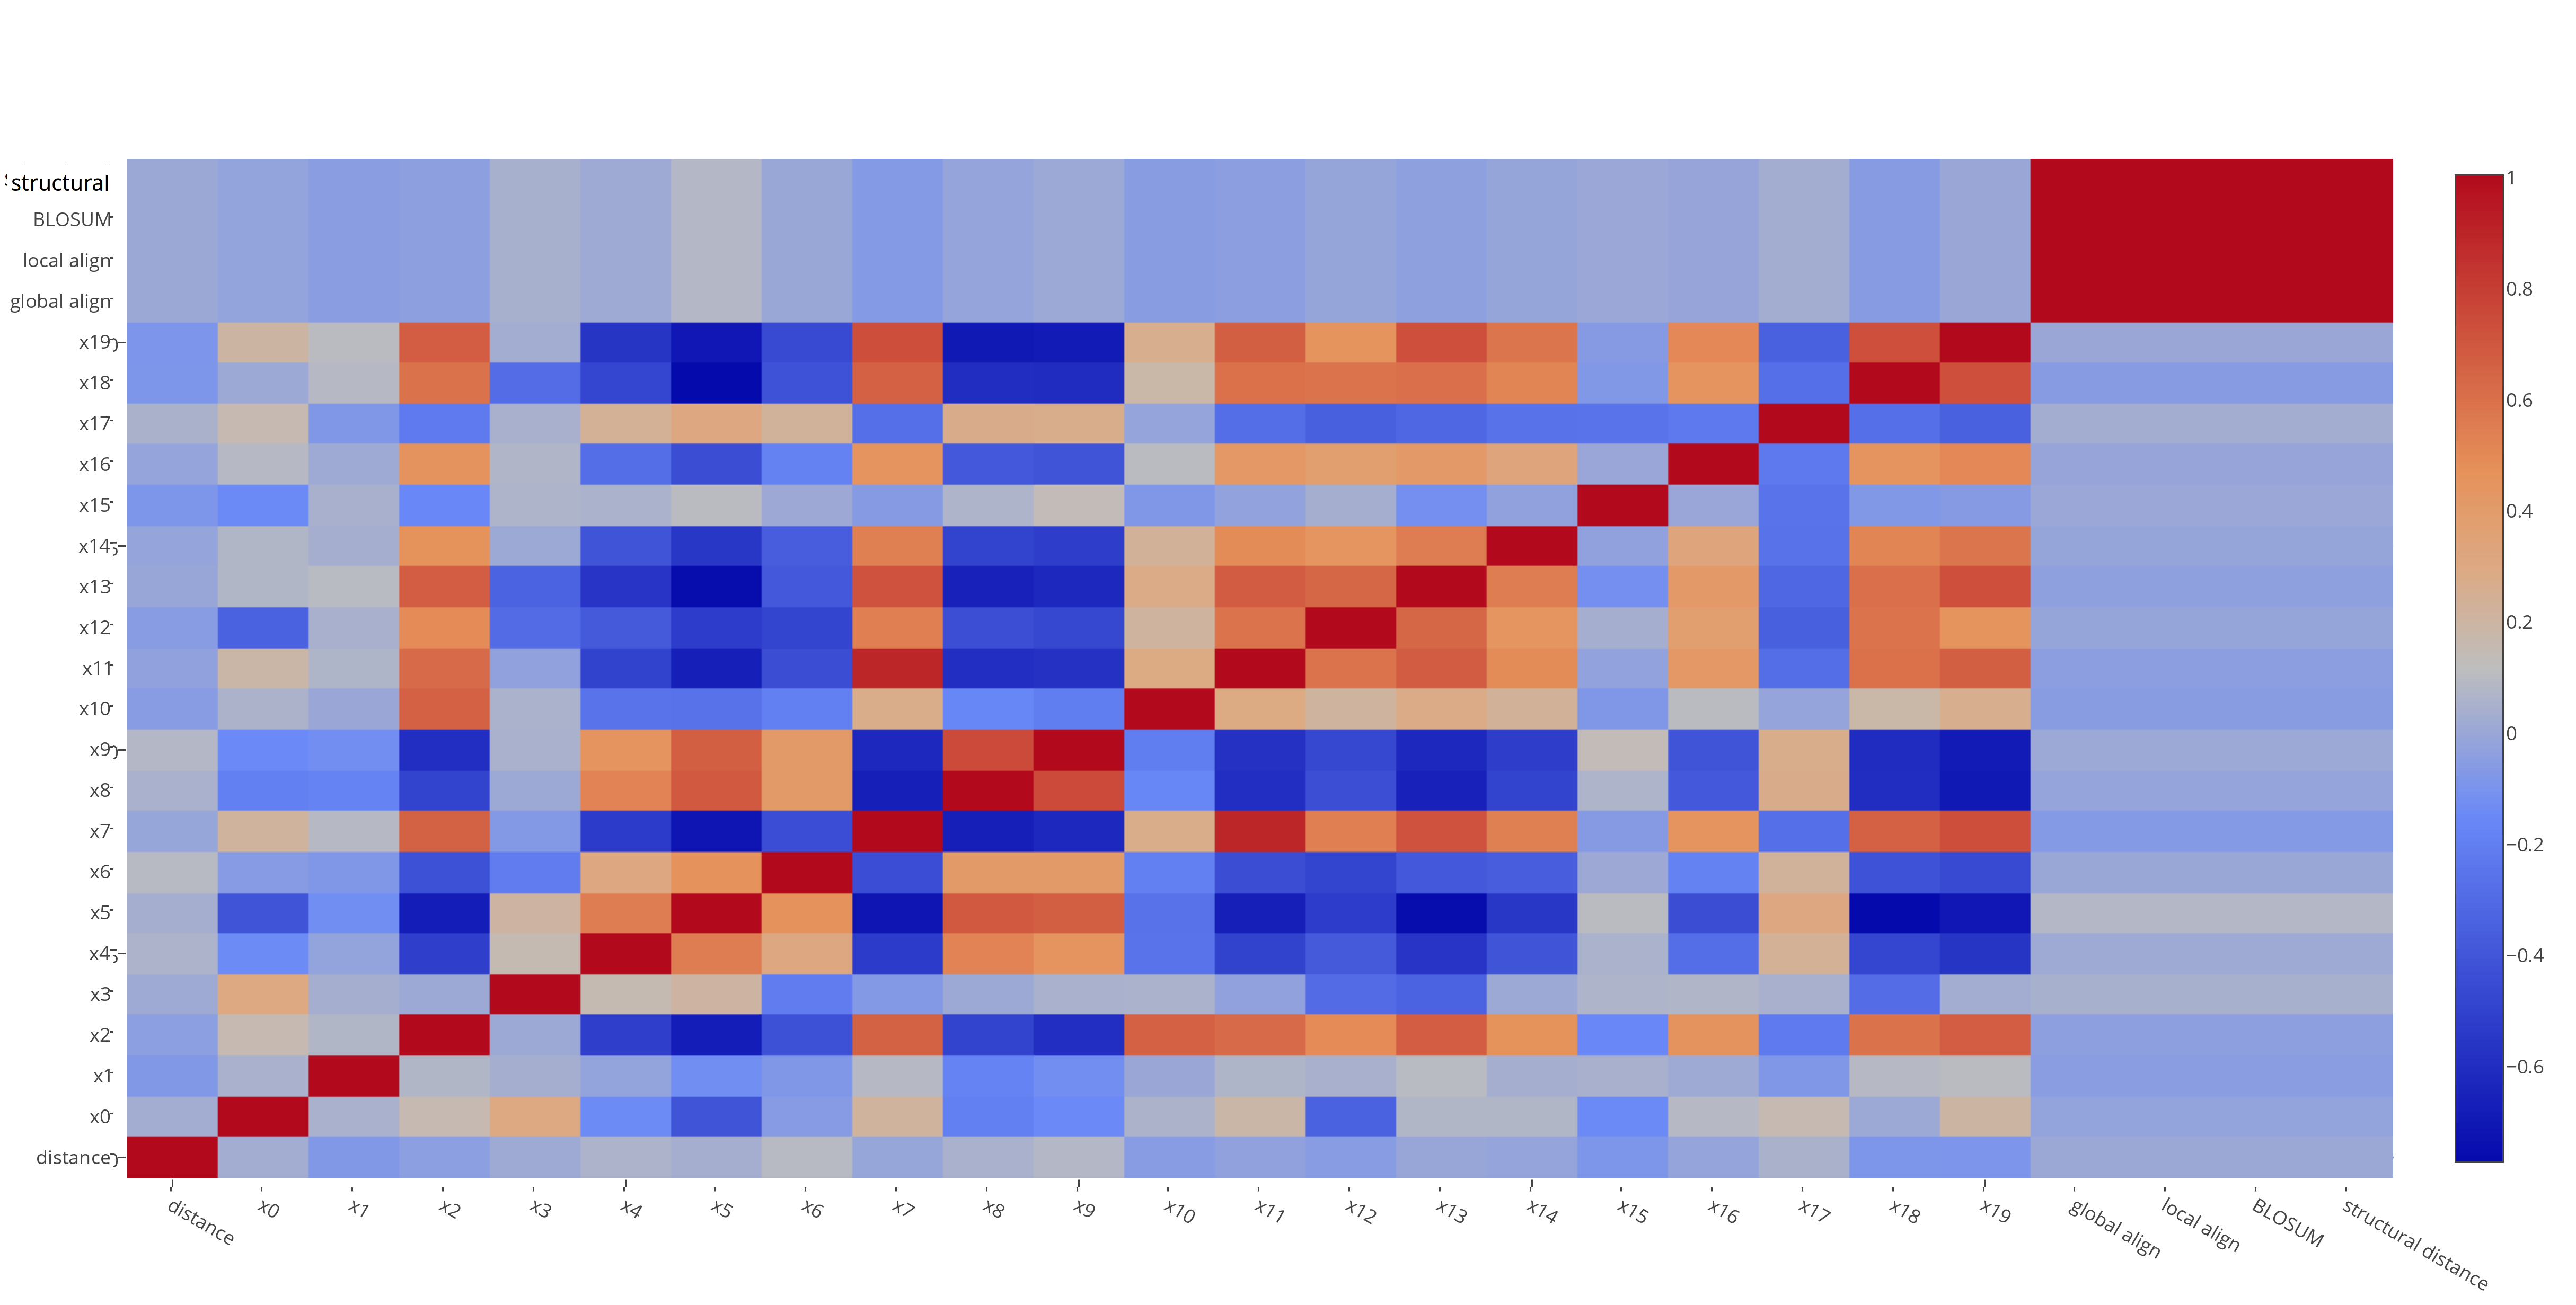
\includegraphics[width=1\textwidth]{PairOneRecHeat}
  \caption{Corrélations pour des paires de fragments avec l'encodeur récurrent
    à représentation one-hot}
\end{figure}

\begin{figure}[H]
  \centering
    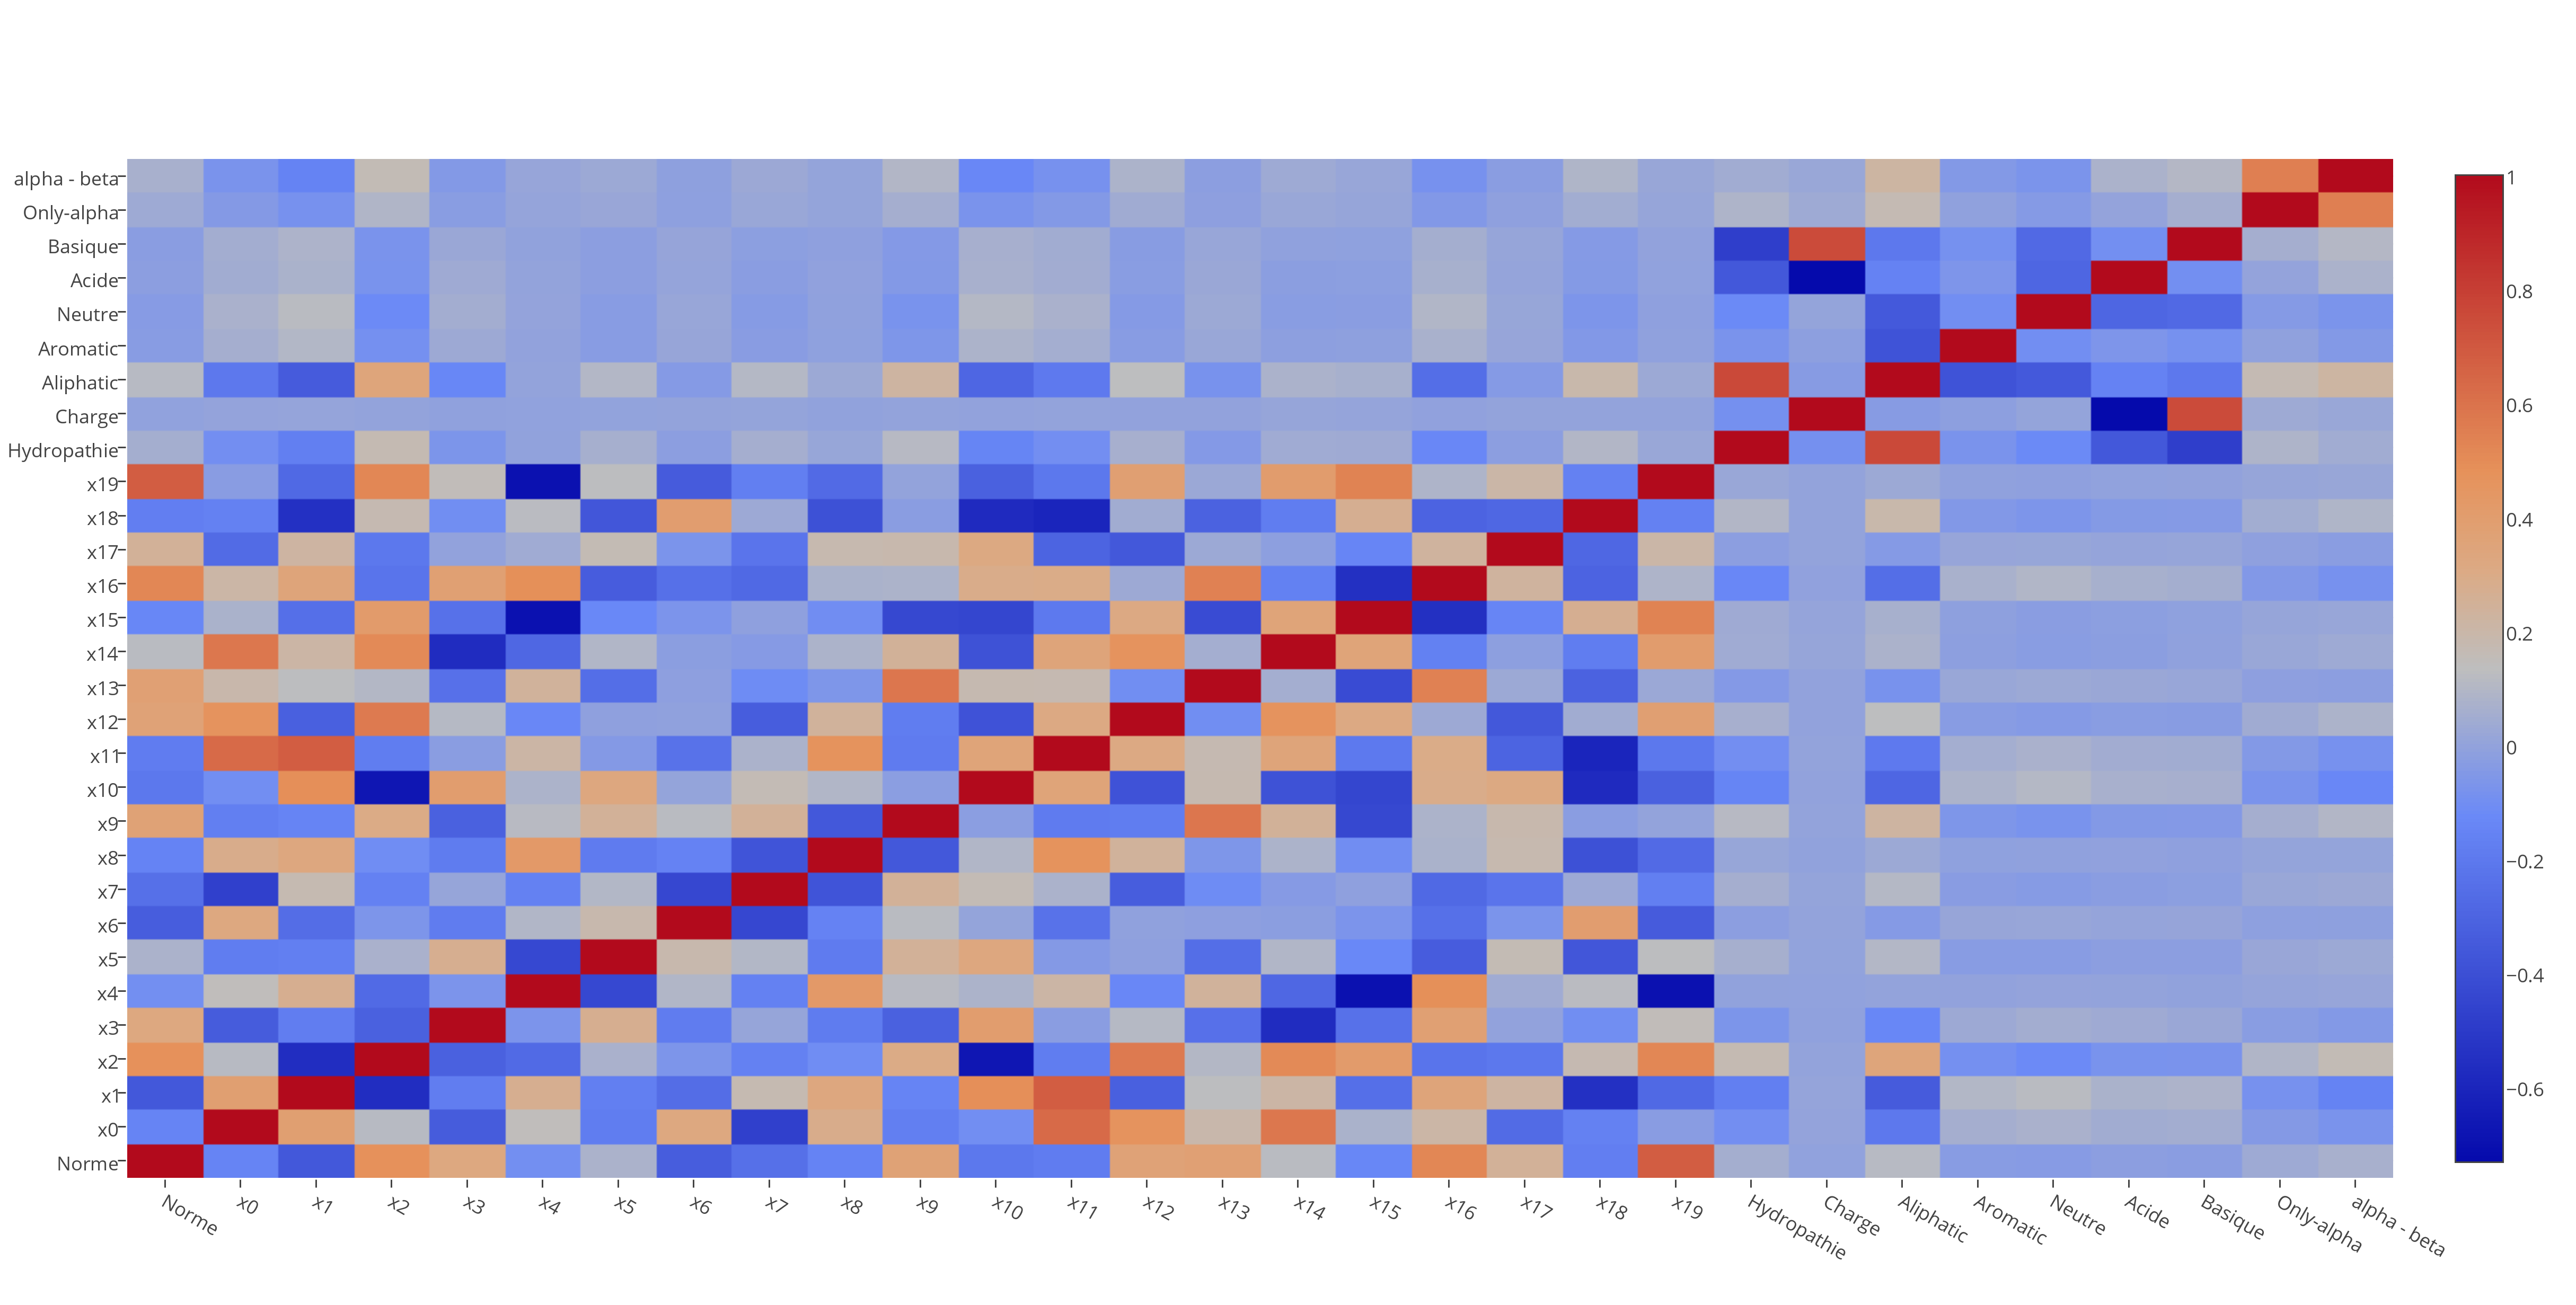
\includegraphics[width=1\textwidth]{SingleOneConvHeat}
    \caption{Corrélations pour des fragments individuels avec l'encodeur convolutionnel
    à représentation one-hot}
\end{figure}

\begin{figure}[H]
  \centering
    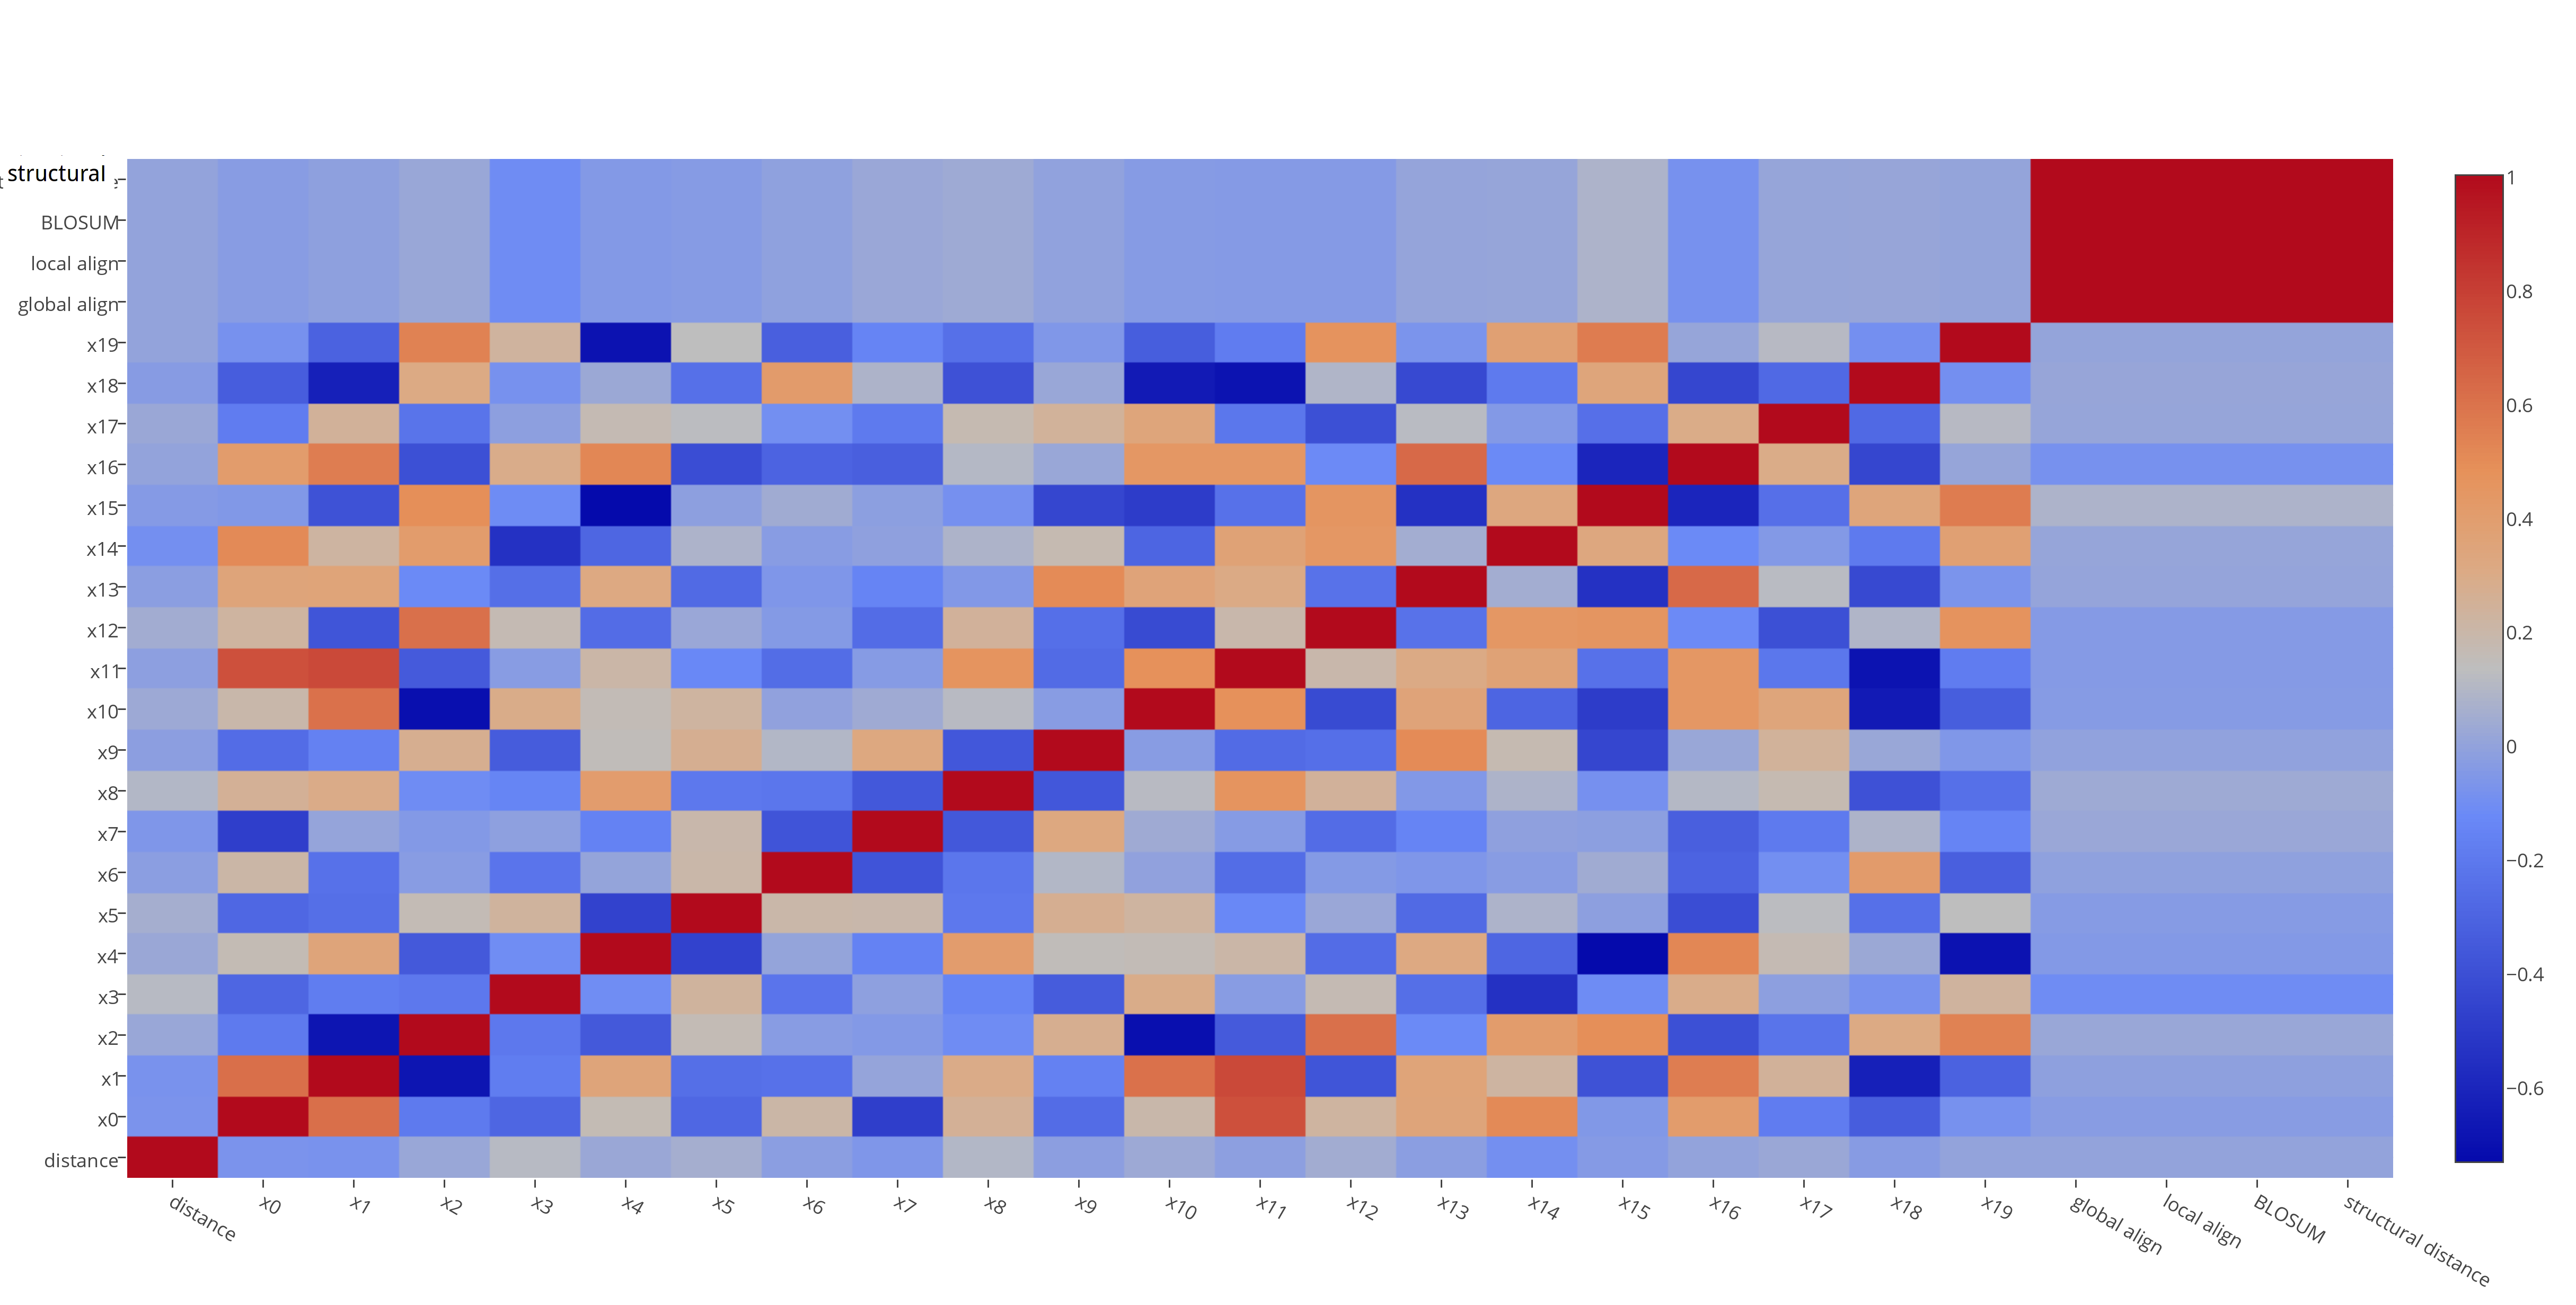
\includegraphics[width=1\textwidth]{PairOneConvHeat}
    \caption{Corrélations pour des paires de fragments avec l'encodeur convolutionnel
      à représentation one-hot}
\end{figure}

\begin{figure}[H]
  \centering
    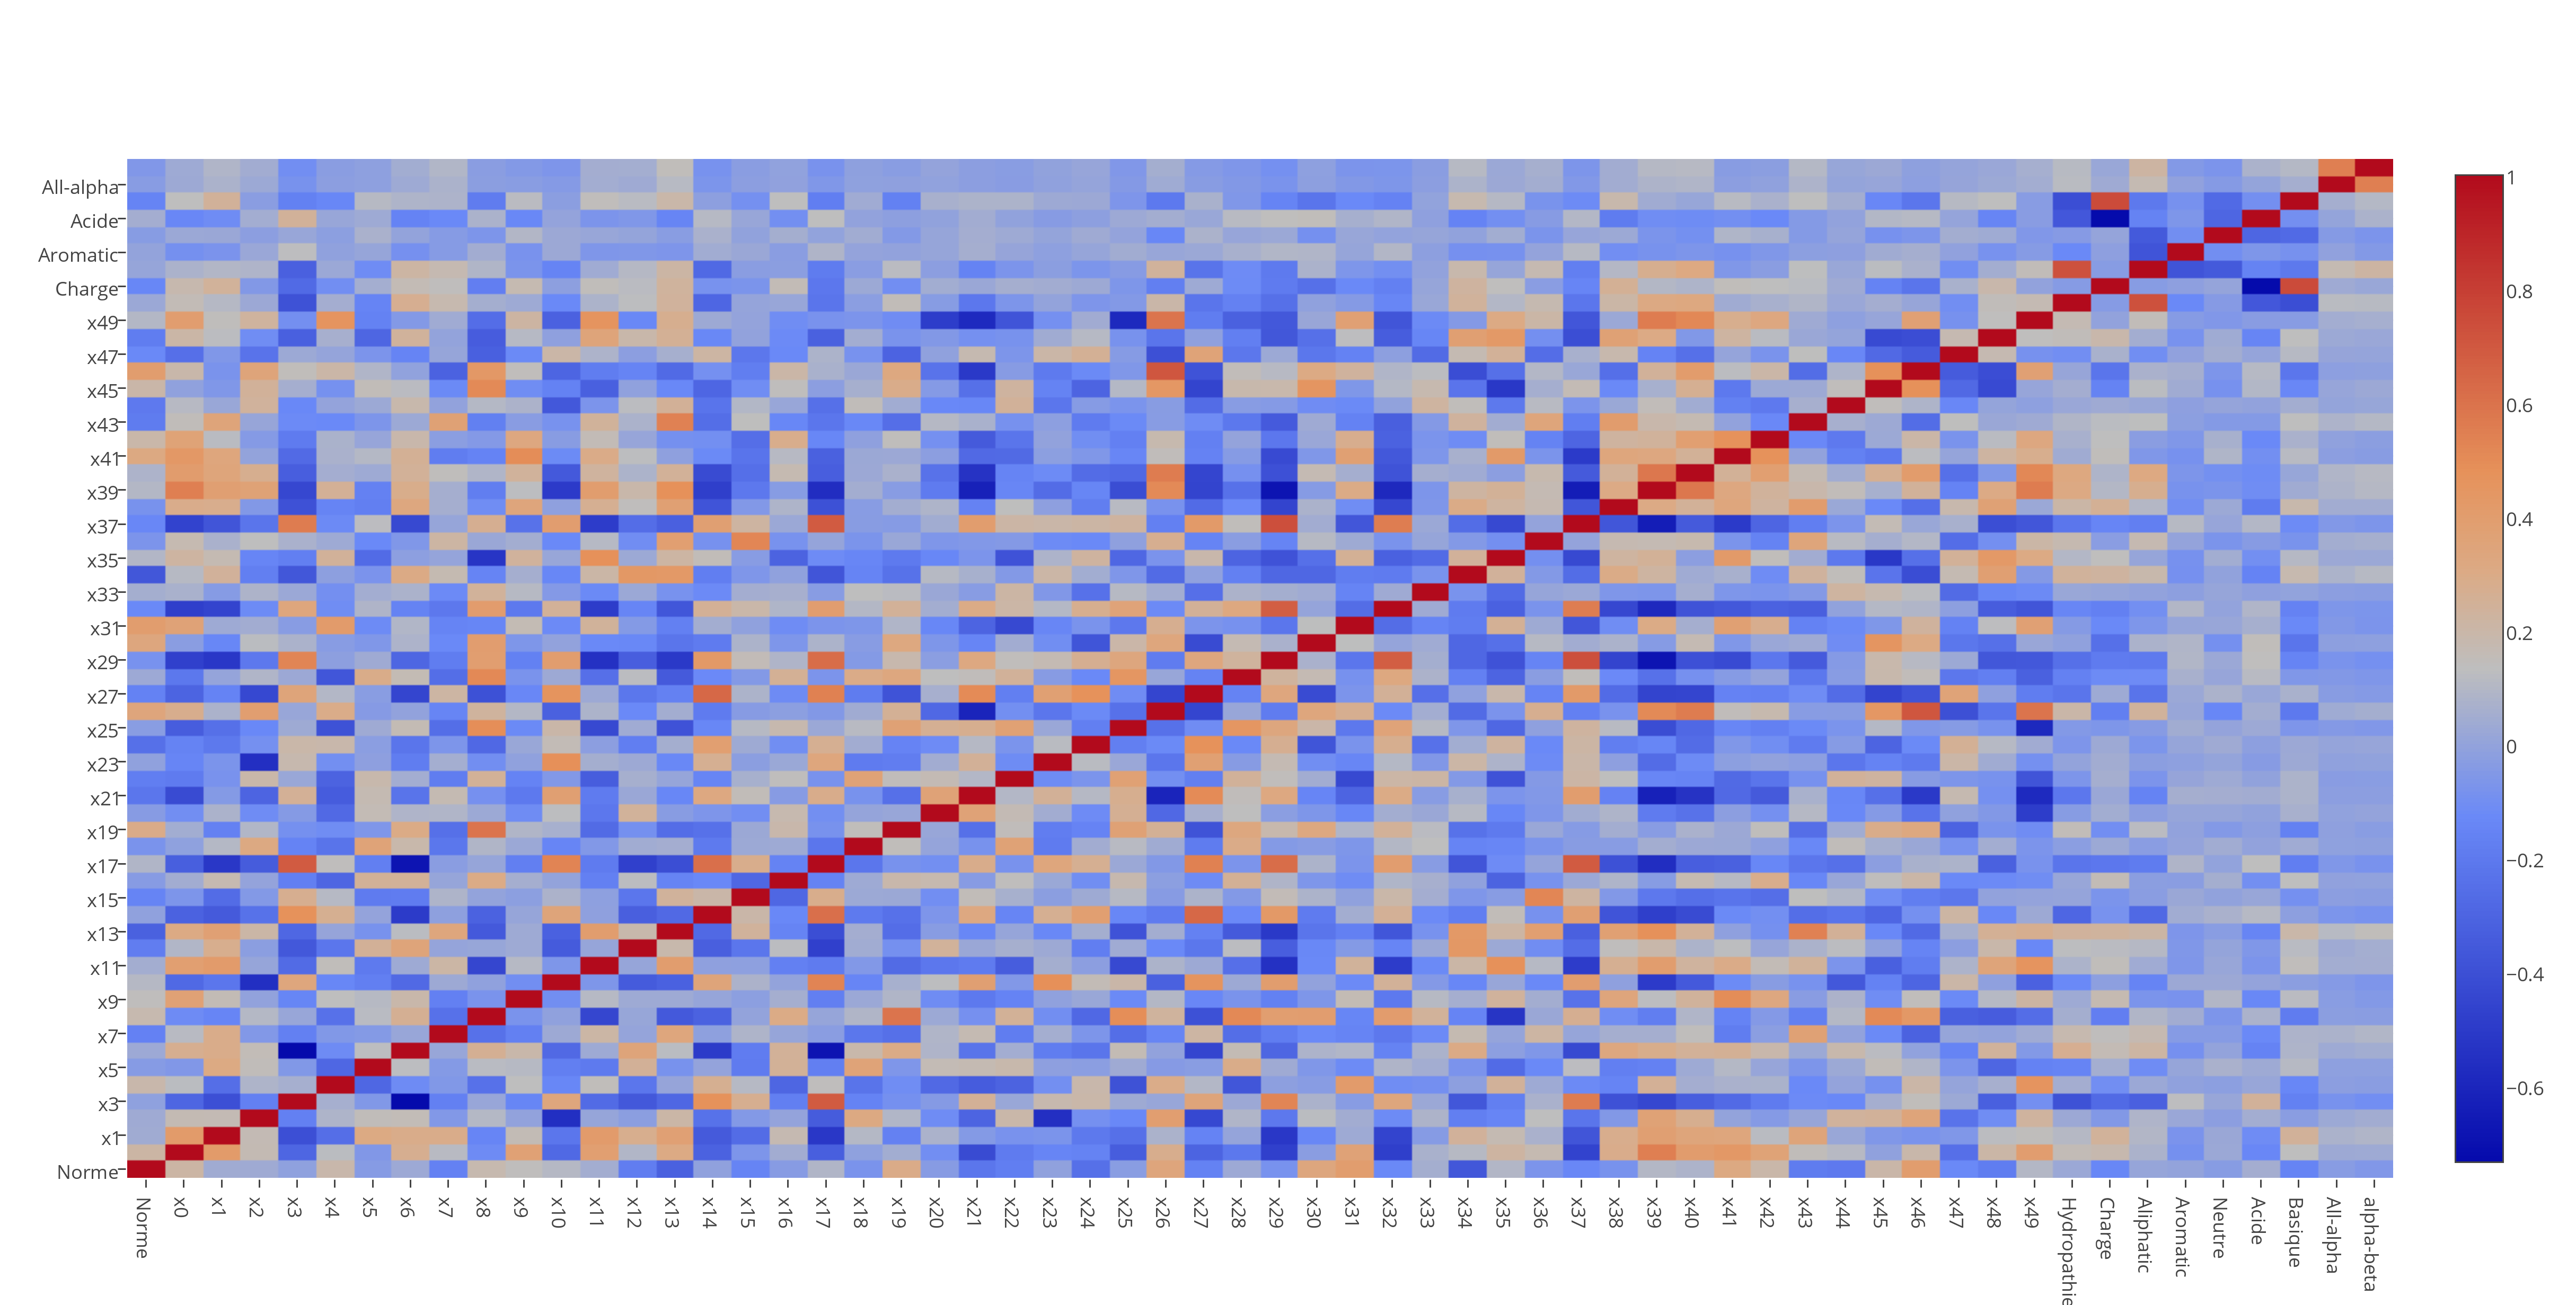
\includegraphics[width=1\textwidth]{SingleEmbedRecHeatf}
    \caption{Corrélations pour des fragments individuels avec l'encodeur récurrent
      à représentation experte}
\end{figure}

\begin{figure}[H]
  \centering
    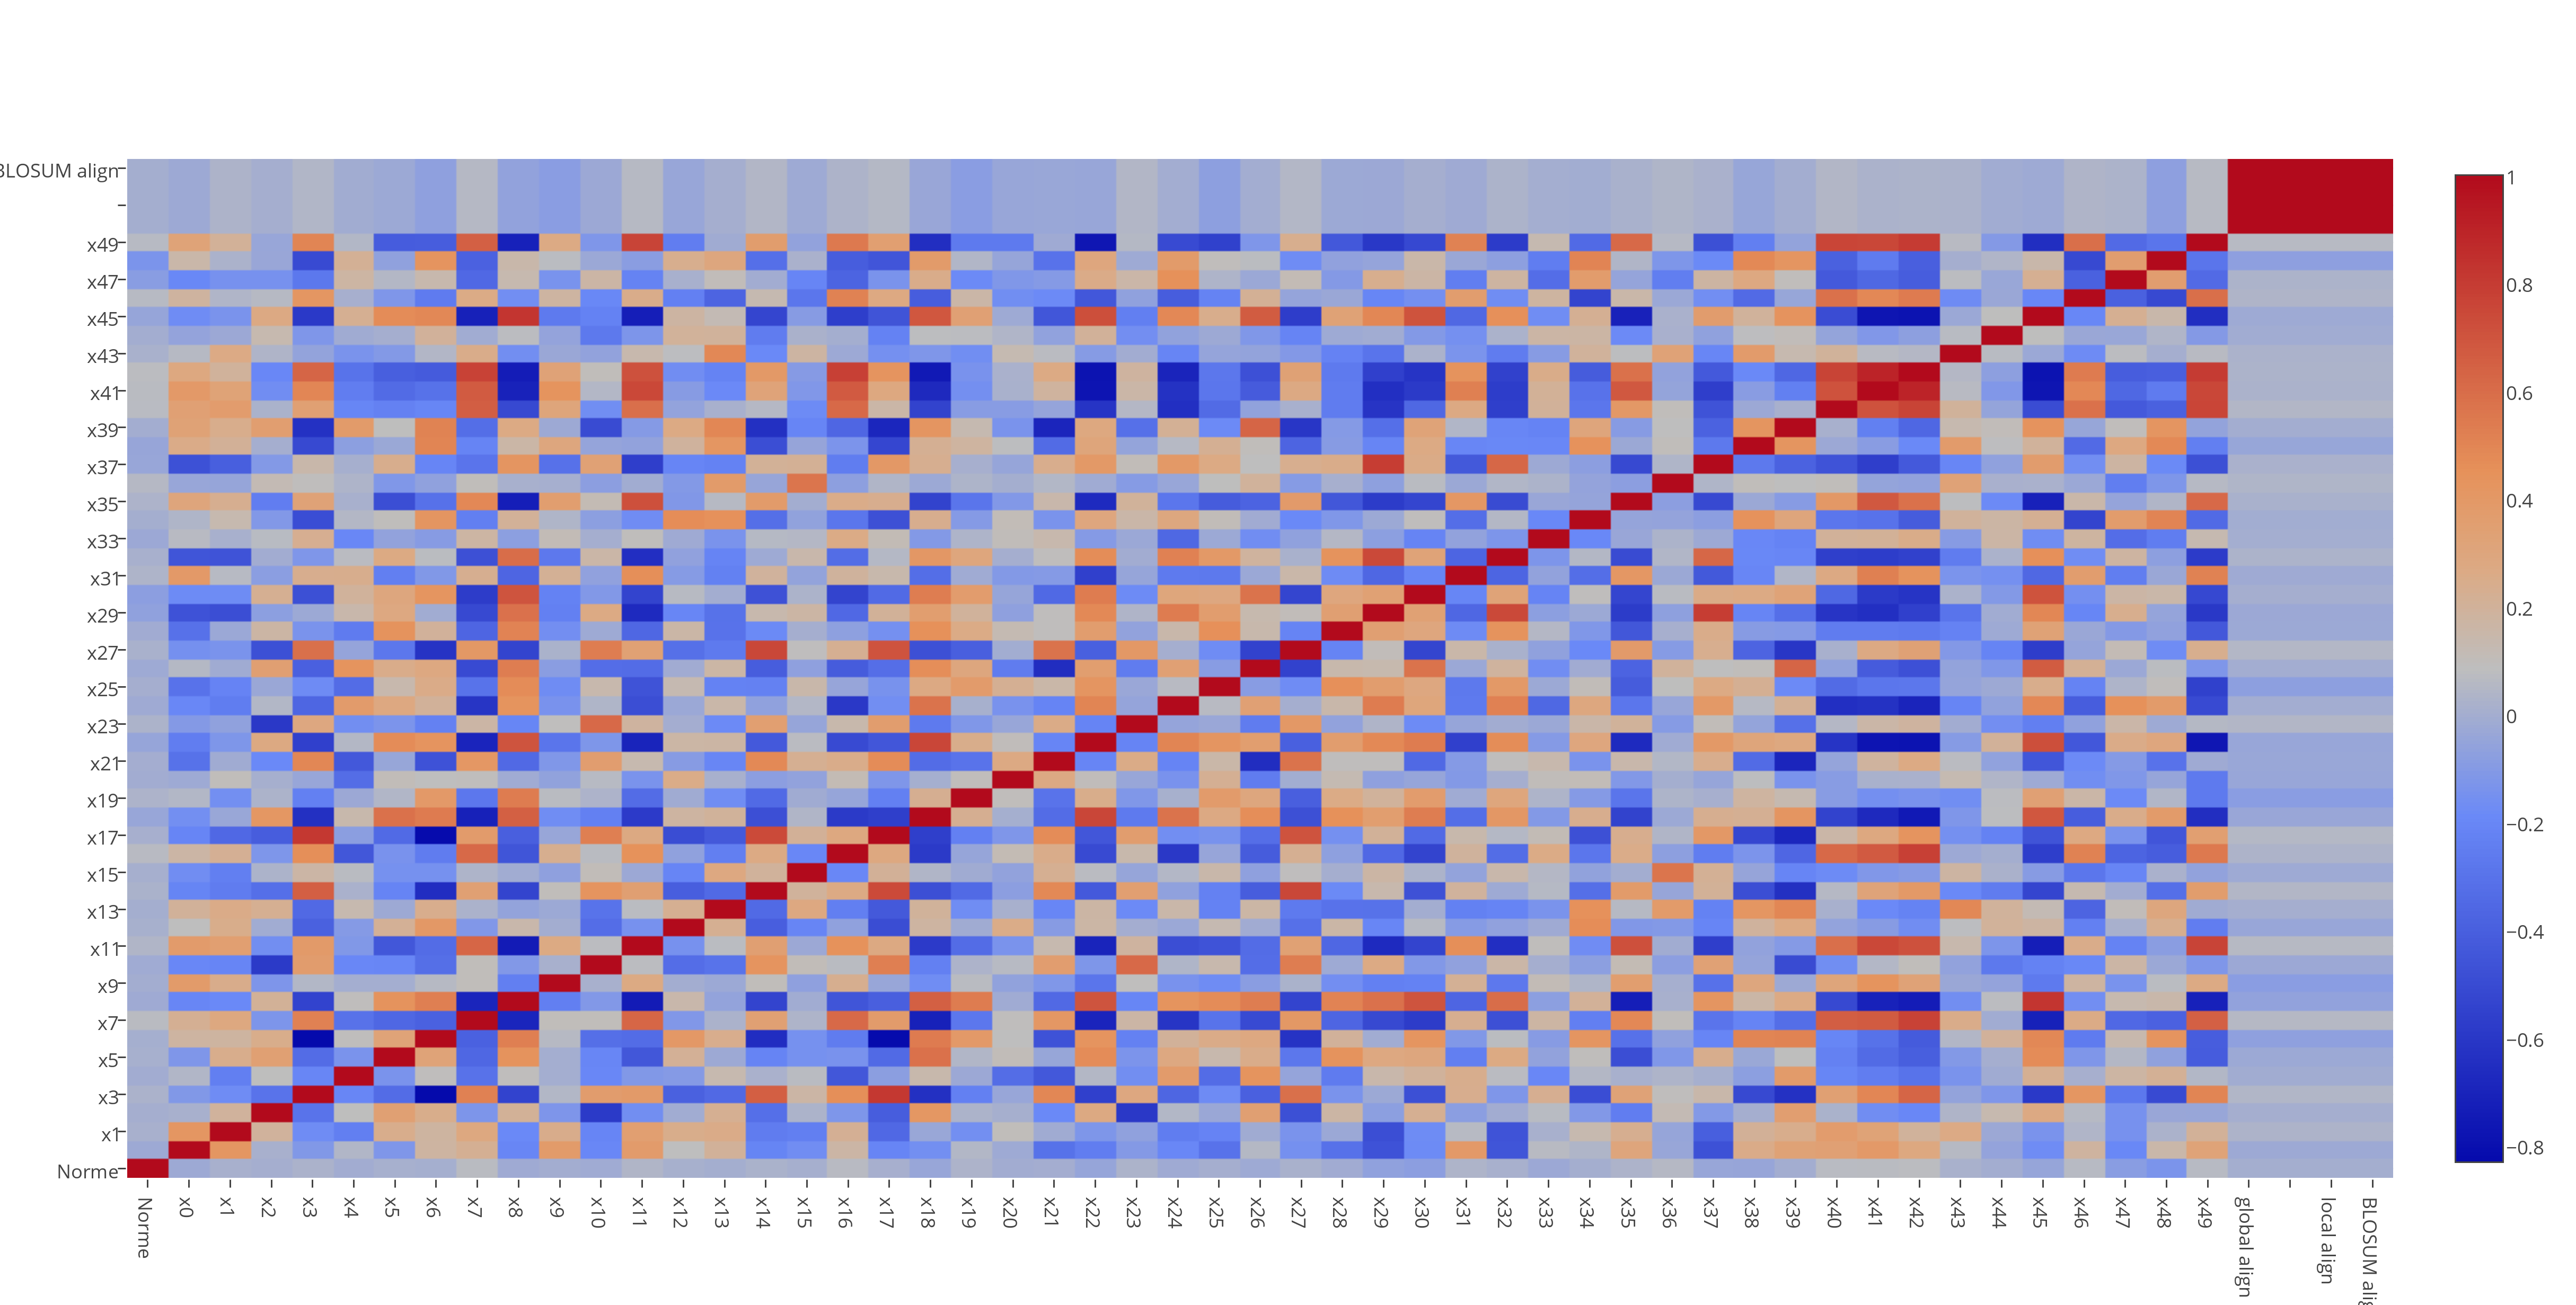
\includegraphics[width=1\textwidth]{PairEmbedRecHeat}
    \caption{Corrélations pour des paires de fragments avec l'encodeur récurrent
      à représentation experte}
\end{figure}

\begin{figure}[H]
  \centering
  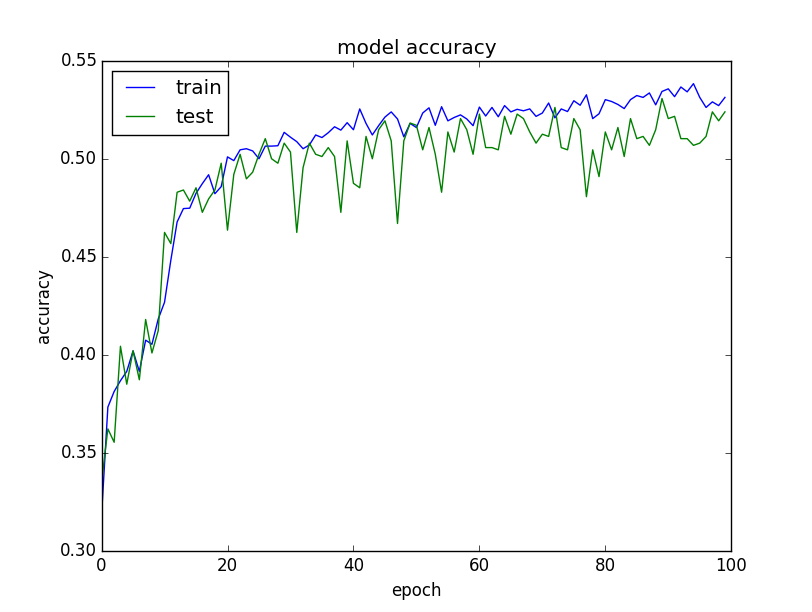
\includegraphics[width=1.1\textwidth]{ConvClass}
  \caption{Classificateur pré-entraîné avec encodeur
    convolutionnel à représentation one-hot}
\end{figure}

\end{document}
